\chapter{修复受损的大脑} \label{chap:chap50}

在其历史的大部分时间里,神经病学一直是一门诊断严谨但疗效甚微的学科。
简而言之,神经学家以其能够非常精确地定位病变而闻名,但直到最近,他们在治疗方面几乎没有什么可提供的。
这种情况现在正在改变。


我们对大脑神经元、神经胶质细胞和突触的结构、功能和化学的理解取得了进展,从而产生了新的治疗思路。
其中许多现在正在进行临床试验,有些已经可供患者使用。
由于三个主要原因,发育神经科学正在成为这种巨变的主要贡献者。
首先,保存或替换因损伤或疾病而丢失的神经元的努力依赖于我们对控制胚胎中神经细胞生成和死亡的机制的理解的最新进展(第~\ref{chap:chap45}~和~\ref{chap:chap46}~章)。
其次,改善损伤后神经通路再生的努力很大程度上依赖于我们对轴突生长和突触形成的了解(第~\ref{chap:chap47}~和~\ref{chap:chap48}~章)。
第三,越来越多的证据表明,一些破坏性脑部疾病,如孤独症和精神分裂症,是胚胎或出生后早期神经回路形成障碍的结果。
因此,对正常发育的研究为准确发现疾病出了什么问题提供了必要的基础。


在本章中,我们将关注其中的前两个问题:神经科学家希望如何增强神经元的有限能力以恢复正常功能。
我们将从描述轴突及其末端与细胞体分离后轴突如何退化开始。
切断的轴突的再生在哺乳动物的周围神经系统和低等脊椎动物的中枢神经系统中是强大的,但在哺乳动物的中枢神经系统中非常差。
许多研究人员都在寻找这些差异的原因,希望通过理解它们能够找到促进人脑和脊髓损伤后恢复的方法。
事实上,我们将看到哺乳动物神经元再生能力的几个差异已经被发现,每一个差异都开辟了有前途的新治疗方法。


然后我们将考虑神经损伤的一个更可怕的后果:神经元的死亡。
成人大脑无法形成新神经元一直是神经科学的中心教条,因为先驱神经解剖学家\textit{圣地亚哥$\cdot$拉蒙-卡哈尔}断言,在受损的中枢神经系统中,“一切都可能死亡,没有任何东西可以再生。” 
尽管\textit{拉蒙-卡哈尔}补充说:“如果可能的话,未来的科学将改变这一严厉的法令,但在上个世纪的大部分时间里,这种悲观的观点主导了神经学。”
值得注意的是,在过去的几十年里,越来越多的证据表明神经发生确实发生在成年哺乳动物大脑的某些区域。
这一发现有助于加快研究刺激神经发生和替换损伤后神经元的方法的步伐。
一个多世纪后,神经科学家终于开始推翻卡哈尔的“严厉法令”。



\section{轴突的损伤会影响神经元和邻近细胞}

由于许多神经元有很长的轴突和中等大小的细胞体,对中枢或外周神经系统的大多数损伤都涉及轴突的损伤。
通过切割或挤压的方式切断轴突被称为轴突切断术,其后果有很多。

\subsection{轴突变性是一个活跃的过程}

轴突切开术将轴突一分为二:
一个仍然附着在细胞体上的近端部分和一个失去了这一关键附着点的远端部分。
轴突切开术破坏了轴突的远端部分,因为在短暂的潜伏期能量供应减少。
很快,改变就变得不可逆转了。
切断的神经末梢的突触传递失败,轴突内的钙水平增加。
钙激活蛋白酶,启动细胞骨架分解和降解程序,随后发生轴突的物理退化。
一旦去神经支配开始,其进展相对较快并且不可避免地进行至完成(图~\ref{fig:50_1})。
这种退化反应是精心设计的一系列变化中的第一步,称为沃勒变性,奥古斯都沃勒最初于 1850 年对其进行了描述。


\begin{figure}[htbp]
	\centering
	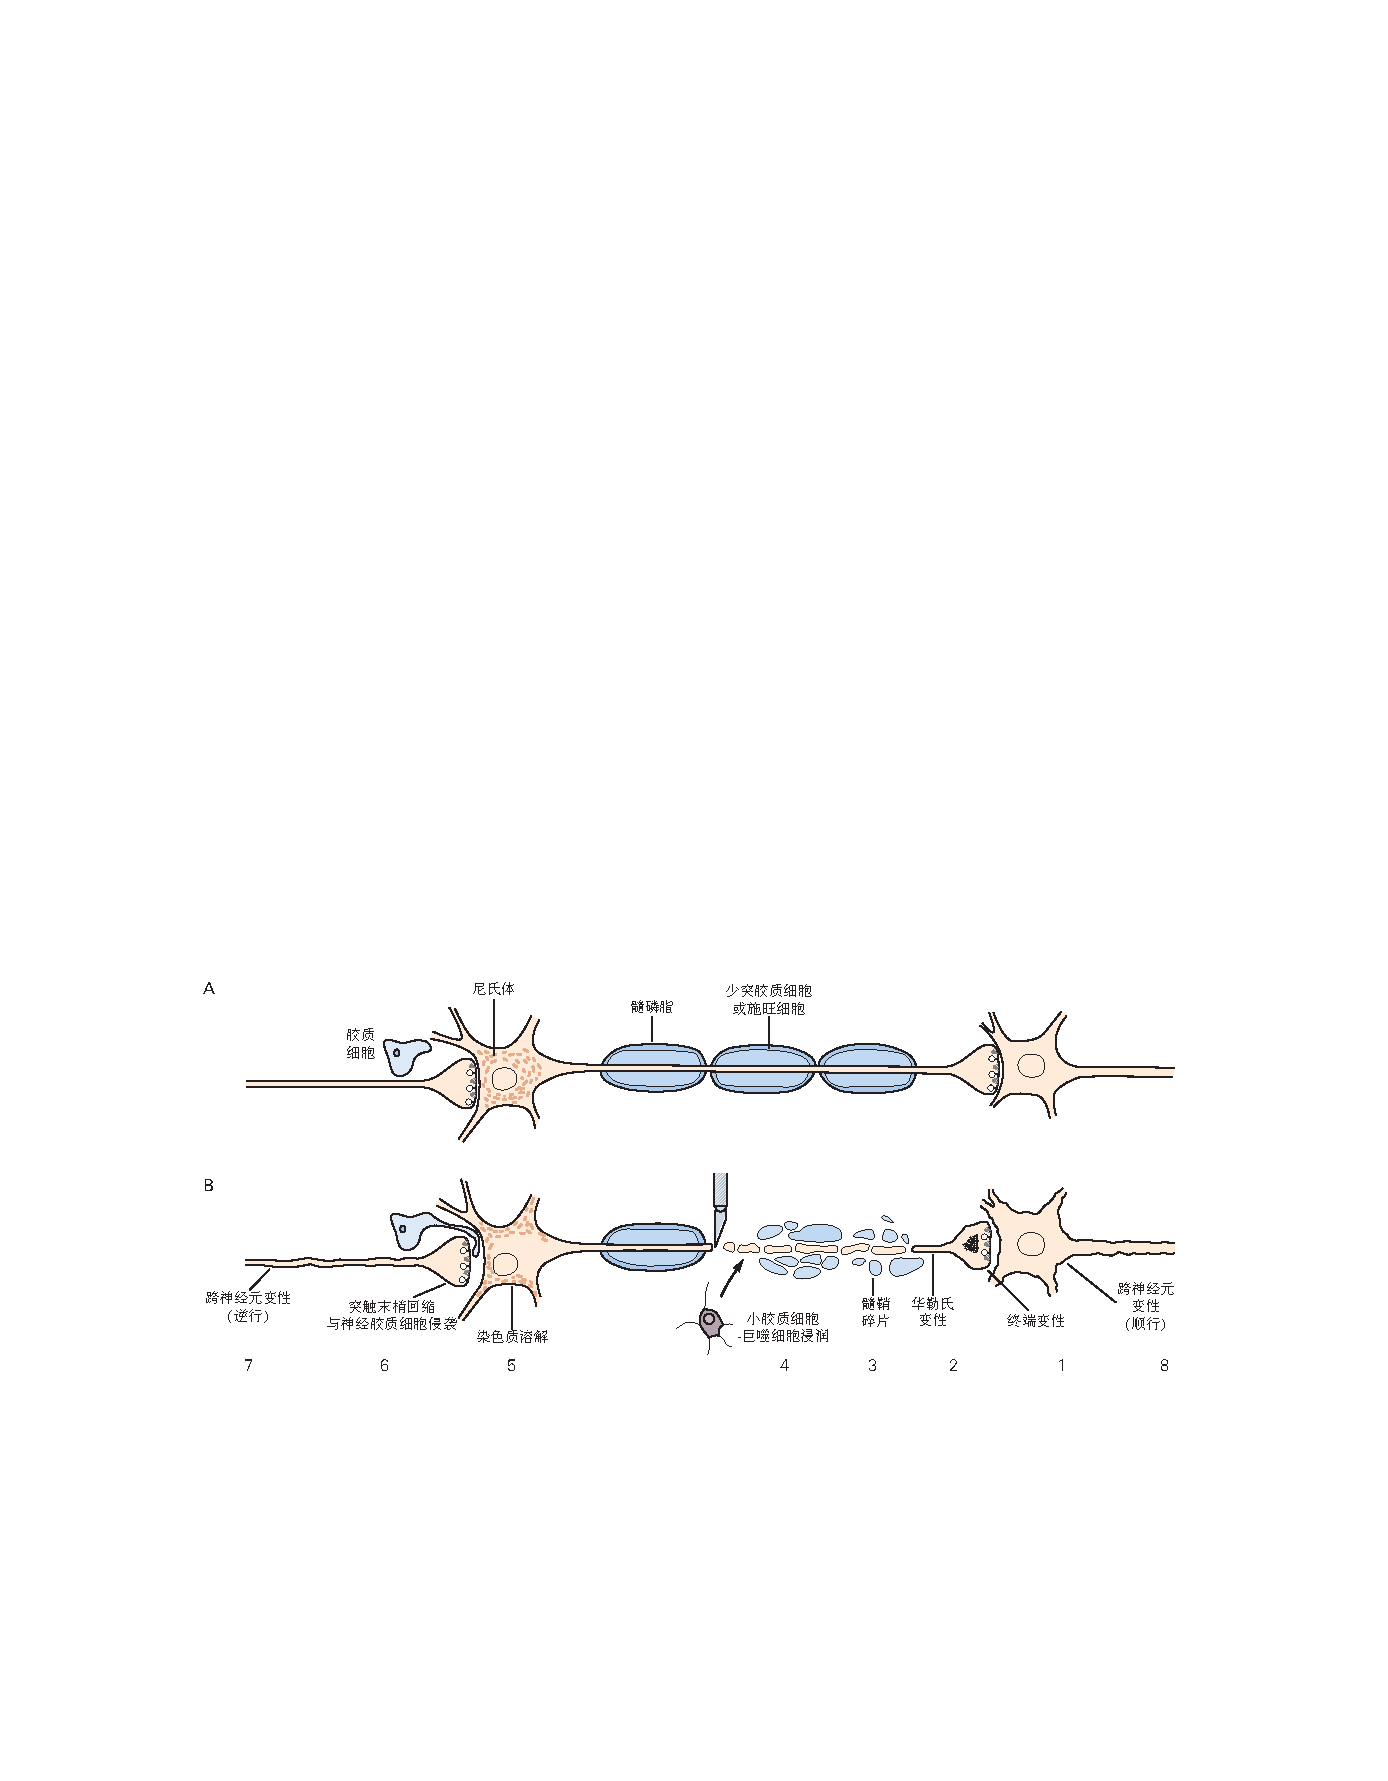
\includegraphics[width=1.0\linewidth]{chap50/fig_50_1}
	\caption{轴突切开术影响受伤的神经元及其突触伙伴。
		\textbf{A.} 具有完整功能轴突并被髓鞘形成细胞包裹的正常神经元与突触后神经元接触。
		神经元的细胞体本身就是一个突触后目标。
		\textbf{B.} 轴索切断术后,受损神经元的神经末梢开始退化(1)。
		远端轴突残端与亲代细胞体分离,变得不规则,并发生沃勒变性(2)。
		髓磷脂开始碎裂(3),病变部位被吞噬细胞侵入(4)。
		受损神经元的细胞体发生色谱分解:细胞体膨胀,细胞核移动到偏心位置(5)。
		与受损神经元接触的突触末端退出,突触部位被神经胶质细胞突侵入(6)。
		受损神经元的输入(7)和目标(8)会萎缩和退化。}
	\label{fig:50_1}
\end{figure}


长期以来,横切轴突的退化被认为是一个被动过程,是与细胞体分离的结果,细胞体的大部分蛋白质都是在细胞体中合成的。
由于缺乏新蛋白质来源,远端残肢被认为会枯萎。
但是在小鼠中发现和分析了一种称为\textit{华勒氏慢变性}的自发突变,对这种观点提出了挑战(图~\ref{fig:50_2})。 
在\textit{华勒氏慢变性}突变小鼠中,周围神经的远端残端在横断后持续存在数周,比正常小鼠长约 10 倍。
这一非凡的发现表明,退化不是与细胞体分离的被动结果,而是一种主动调节的反应。


\begin{figure}[htbp]
	\centering
	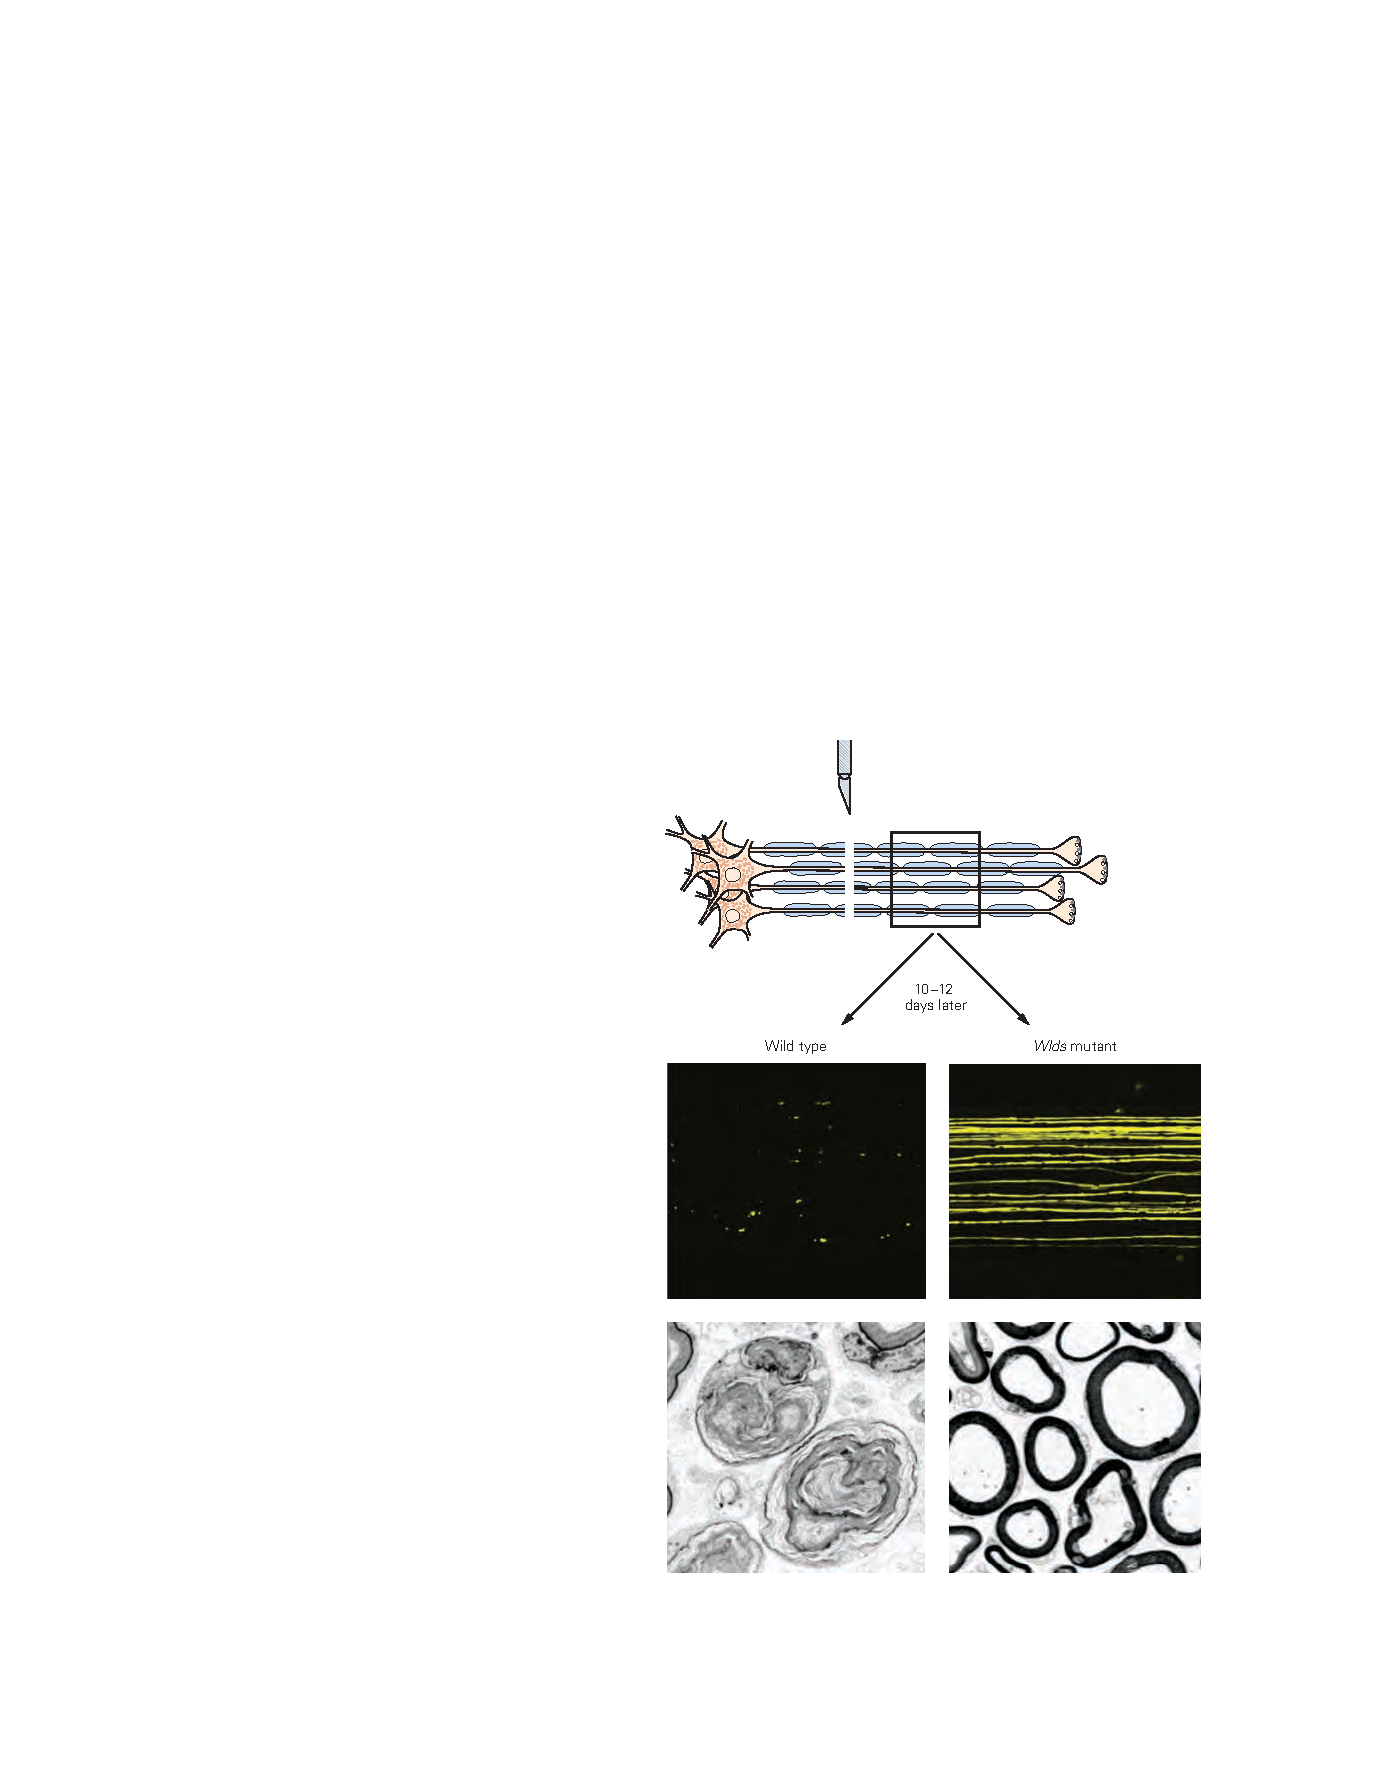
\includegraphics[width=0.71\linewidth]{chap50/fig_50_2}
	\caption{\textit{华勒氏慢变性}突变小鼠的轴突变性延迟。
		在野生型动物中,远端残端的轴突在周围神经切片后迅速退化,如轴突碎片(黄色)中断和电子显微水平上缺乏髓鞘轴突轮廓所示。
		在\textit{华勒氏慢变性}突变小鼠中,切断轴突的远端部分会持续很长时间\cite{beirowski2004quantitative}。}
	\label{fig:50_2}
\end{figure}


对\textit{华勒氏慢变性}突变小鼠的分析导致了对该法规性质的深入了解。
该突变导致形成突变形式的\textit{烟酰胺单核苷酸腺嘌呤转移酶1},这是一种参与代谢辅因子\textit{烟酰胺腺嘌呤二核苷酸}生物合成的酶。
通常存在于轴突中的相关酶\textit{烟酰胺单核苷酸腺嘌呤转移酶2}在轴突切开后变得非常不稳定并迅速分解,导致\textit{烟酰胺腺嘌呤二核苷酸}的损失,这对于维持轴突中的能量稳态至关重要。
虽然正常的\textit{烟酰胺单核苷酸腺嘌呤转移酶1}局限于细胞核,但突变的\textit{华勒氏慢变性}形式错误定位到轴突,在那里它替代\textit{烟酰胺单核苷酸腺嘌呤转移酶2}以延长轴突存活。
令人惊讶的是,野生型和\textit{华勒氏慢变性}形式的\textit{烟酰胺单核苷酸腺嘌呤转移酶1}维持\textit{烟酰胺腺嘌呤二核苷酸}水平的主要方式不是通过合成它,而是通过抑制另一种分解\textit{烟酰胺腺嘌呤二核苷酸}的蛋白质 SARM1。
因此,SARM 的缺失可以保护受损的轴突,而 SARM1 的激活会导致退化(图~\ref{fig:50_3}A)。
其他几种蛋白质调节该核心通路(图~\ref{fig:50_3}B)。


\begin{figure}[htbp]
	\centering
	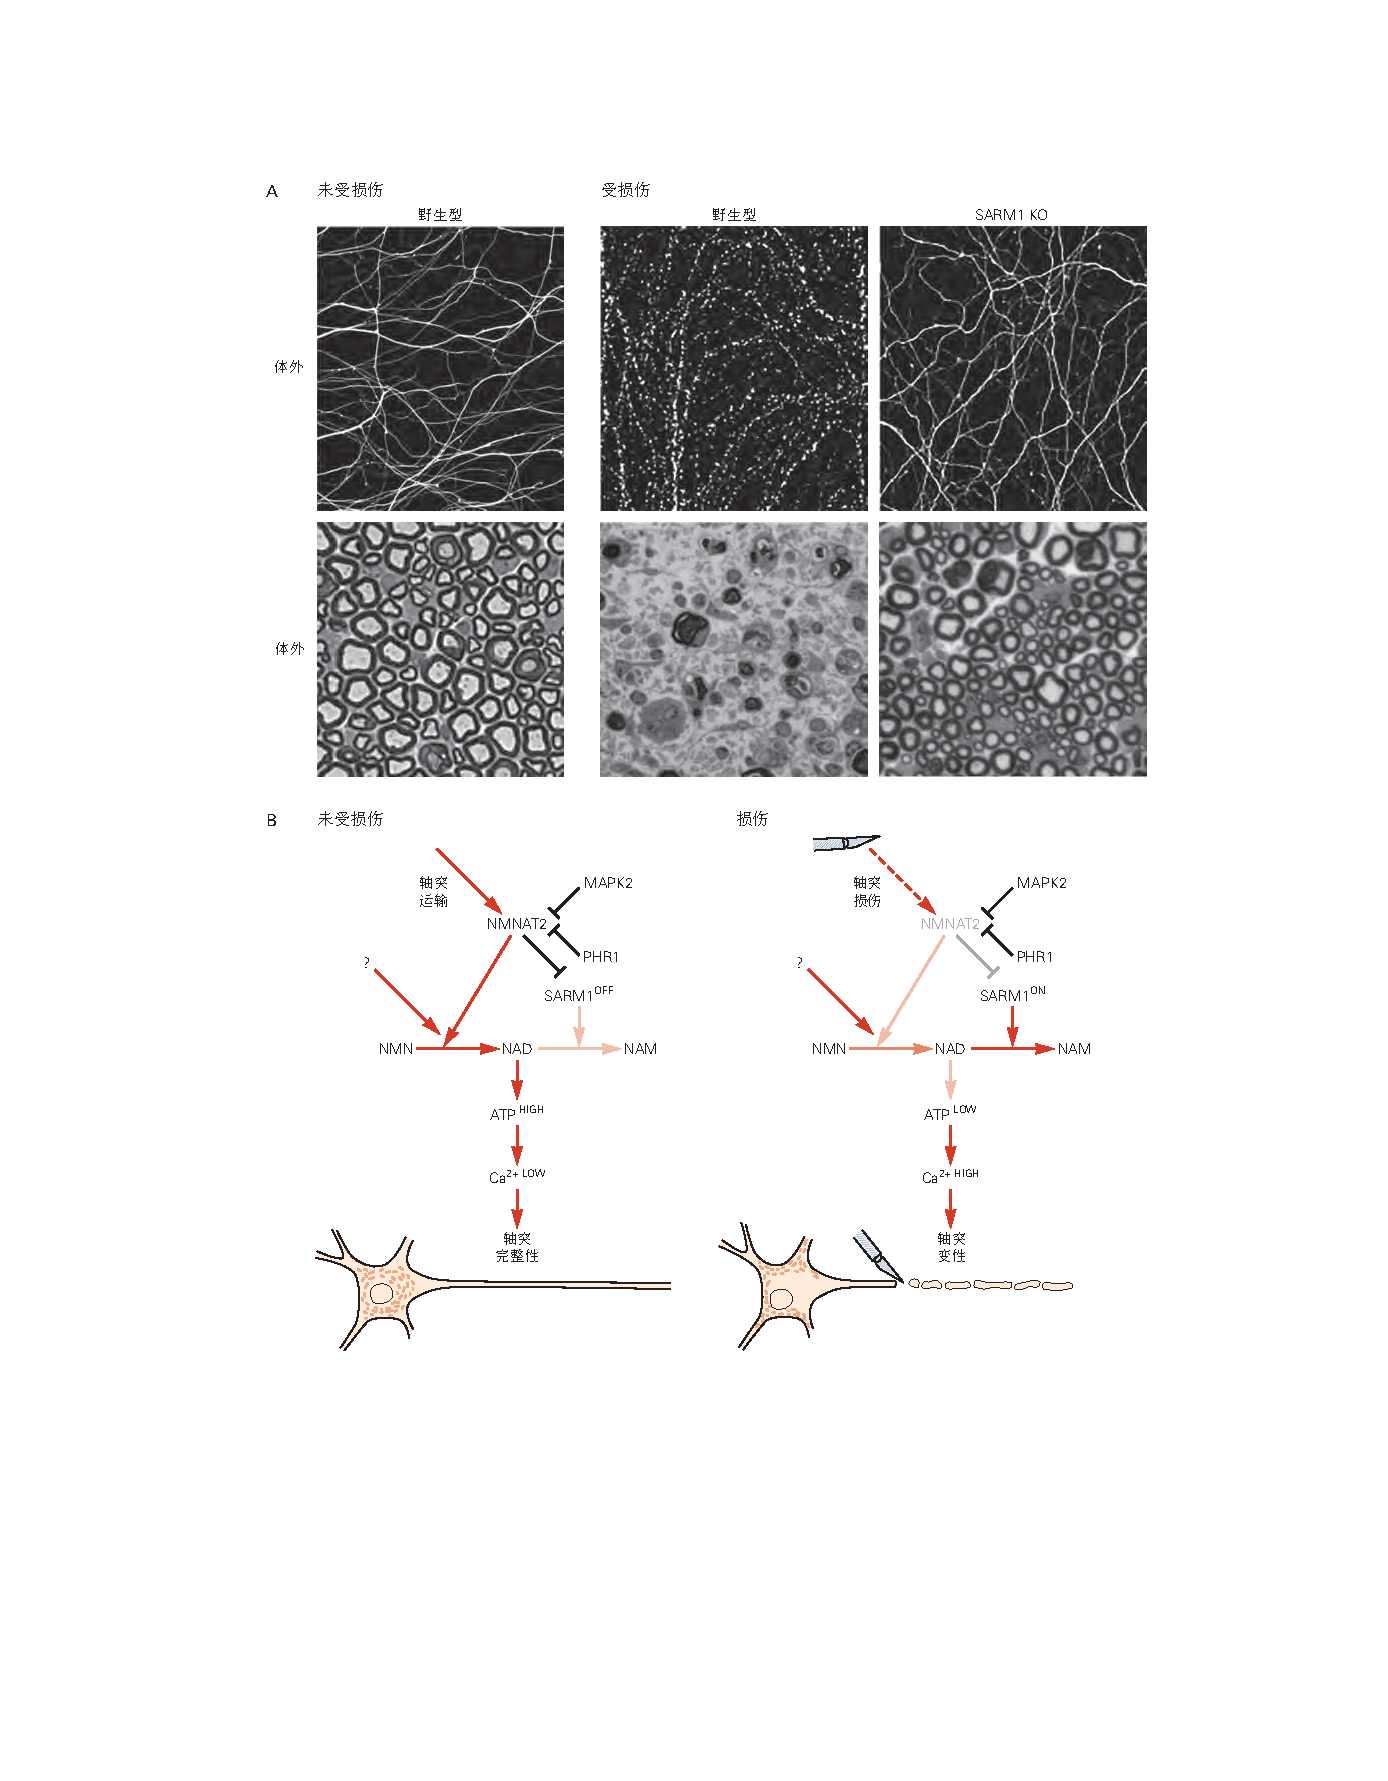
\includegraphics[width=0.97\linewidth]{chap50/fig_50_3}
	\caption{一条核心通路调节小鼠轴索切断术后的轴突变性。
		\textbf{A.} 体外神经突损伤导致与细胞体分离的部分变性。
		同样,体内轴突切开术导致沃勒变性,如横截面中髓鞘轮廓的丢失所示。
		如果 SARM1 基因被删除,体外和体内的轴突都会幸免。
		\textbf{B.} \textit{烟酰胺单核苷酸腺嘌呤转移酶2}与突变体\textit{华勒氏慢变性}蛋白密切相关,通常存在于轴突中。
		它可以生成\textit{烟酰胺腺嘌呤二核苷酸}并抑制降解\textit{烟酰胺腺嘌呤二核苷酸}的 SARM1。
		能量代谢需要高\textit{烟酰胺腺嘌呤二核苷酸}水平,从而使轴突中的\textit{三磷酸腺苷}水平保持高水平,钙水平保持低水平。
		轴突切开后,\textit{烟酰胺单核苷酸腺嘌呤转移酶2}水平迅速下降,从而抑制 SARM1。
		\textit{烟酰胺腺嘌呤二核苷酸}水平下降,\textit{三磷酸腺苷}耗尽,钙水平升高,钙依赖性蛋白酶被激活,轴突被降解。
		\textit{有丝分裂原活化蛋白激酶}和泛素连接酶(Phr1)调节该通路。}
	\label{fig:50_3}
\end{figure}


总之,这些激动人心的新发现为以下问题提供了答案:
为什么在轴突切开术后,远端残端退化而近端残端得以保留。
远端残端被剥夺了通常从细胞体输送的营养物质的传统解释是不完整的。
相反,轴突中的信号通路会感知损伤并迅速引发退化。
在这种情况下,轴突提供的关键元素是\textit{烟酰胺单核苷酸腺嘌呤转移酶2}。
它在轴突切开后的分解会抑制 SARM1,并且可能与刺激 SARM1 的因子激活同时发生,从而引发\textit{烟酰胺腺嘌呤二核苷酸}的损失,从而导致能量危机,从而导致沃勒变性。


这些最近的发现可能有助于设计治疗神经系统疾病的方法,在这些疾病中,轴突变性很明显并且通常先于神经元死亡。
运动神经元的致命疾病,肌萎缩侧索硬化症,就属于这一类。
其他可能性包括某些形式的脊髓性肌萎缩症、帕金森病,甚至阿尔茨海默病。
在这些疾病中以及在代谢、毒性或炎症损伤后发生的轴突退化类似于急性创伤后的退化,并且可能以类似的方式进行调节。
因此,虽然保存横断的远端轴突的方法不太可能在临床上用于治疗遭受外伤的患者,但相同的技术可用于治疗神经退行性疾病。


即使轴突的近端部分仍然附着在细胞体上,它也会受到影响。
在某些情况下,神经元本身会因细胞凋亡而死亡,这可能是因为轴突切开术将细胞体与其靶源性营养因子的供应隔离开来。
即使这没有发生,细胞体也经常会经历一系列称为色谱分解反应的细胞和生化变化:
细胞体膨胀,细胞核移动到偏心位置,粗面内质网变得支离破碎(图~\ref{fig:50_1}B)。
色谱分解伴随着其他代谢变化,包括蛋白质和\textit{核糖核酸}合成的增加以及神经元表达的基因模式的变化。
如果重新生成成功,这些更改将被撤销。



\subsection{轴突切开导致附近细胞的反应性反应}

轴突切开术在多种类型的相邻细胞中启动一系列反应。
其中最重要的反应是包裹远端神经节段的神经胶质细胞的反应。
一种是髓鞘破碎,然后被吞噬细胞去除。
这个过程在周围神经系统中很快,产生髓磷脂的雪旺细胞将髓磷脂分解成小碎片并将其吞没。
然后分裂的雪旺细胞分泌从血流中募集巨噬细胞的因子。
巨噬细胞反过来帮助雪旺细胞处理碎片。
雪旺细胞还产生促进轴突再生的生长因子,我们稍后会谈到这一点。


相比之下,在中枢神经系统中,形成髓鞘的少突胶质细胞几乎没有或根本没有处理髓鞘的能力,碎片的清除依赖于称为小胶质细胞的常驻吞噬细胞。
这种细胞特性的差异可能有助于解释观察到的华勒变性在中枢神经系统中进行到完成的速度要慢得多。


轴突切开术还会影响受伤神经元的突触输入和突触目标。
当轴突切开术破坏细胞的主要输入时(就像在去神经肌肉中发生的那样,或者当视神经被切断时在外侧膝状体核中的神经元中发生的情况)后果是严重的。
通常目标会萎缩,有时甚至会死亡。
当目标仅部分去神经时,它们的反应更加有限。
此外,轴突切开术影响突触前神经元。
在许多情况下,突触末端从细胞体或染色质神经元的树突中退出,并被神经胶质细胞的过程所取代(外周的雪旺细胞和中枢神经系统的小胶质细胞或星形胶质细胞)。
这个过程称为突触剥离,会抑制突触活动并会损害功能恢复。


尽管突触剥离的机制仍不清楚,但已提出两种可能性。
一是突触后损伤导致轴突末端失去与突触位点的粘附性,因此它们随后被胶质细胞包裹。
另一个是神经胶质细胞响应受损神经元释放的因子或其细胞表面的变化而启动突触剥离过程。
无论触发因素是什么,轴突切开术对小胶质细胞和星形胶质细胞的激活显然有助于剥离过程。
此外,生化改变的星形胶质细胞,称为反应性星形胶质细胞,有助于在损伤部位附近形成神经胶质疤痕。


由于这些跨突触效应,神经元变性可以在顺行和逆行方向上通过回路传播。
例如,严重萎缩的去神经神经元可能无法激活其目标,从而导致萎缩。
同样,当突触剥离阻止传入神经元从其目标细胞获得足够的营养时,传入神经元的输入就处于危险之中。
这种连锁反应有助于解释中枢神经系统某一区域的损伤最终如何影响远离损伤部位的区域。



\section{受伤后中央轴突再生不良}

中枢神经和外周神经在受伤后的再生能力方面存在很大差异。
外周神经通常可以在受伤后得到修复。
虽然外周轴突的远端节段退化,但远端残端周围的结缔组织元素通常存活下来。


轴突芽从近端残端生长,进入远端残端,并沿着神经向其目标方向生长(图~\ref{fig:50_4})。
驱动这一过程的机制与那些引导胚胎轴突的机制有关。 雪旺细胞分泌的趋化因子将轴突吸引到远端残端,远端残端内的粘附分子促进轴突沿细胞膜和细胞外基质生长,神经鞘中的抑制分子防止再生轴突误入歧途。


\begin{figure}[htbp]
	\centering
	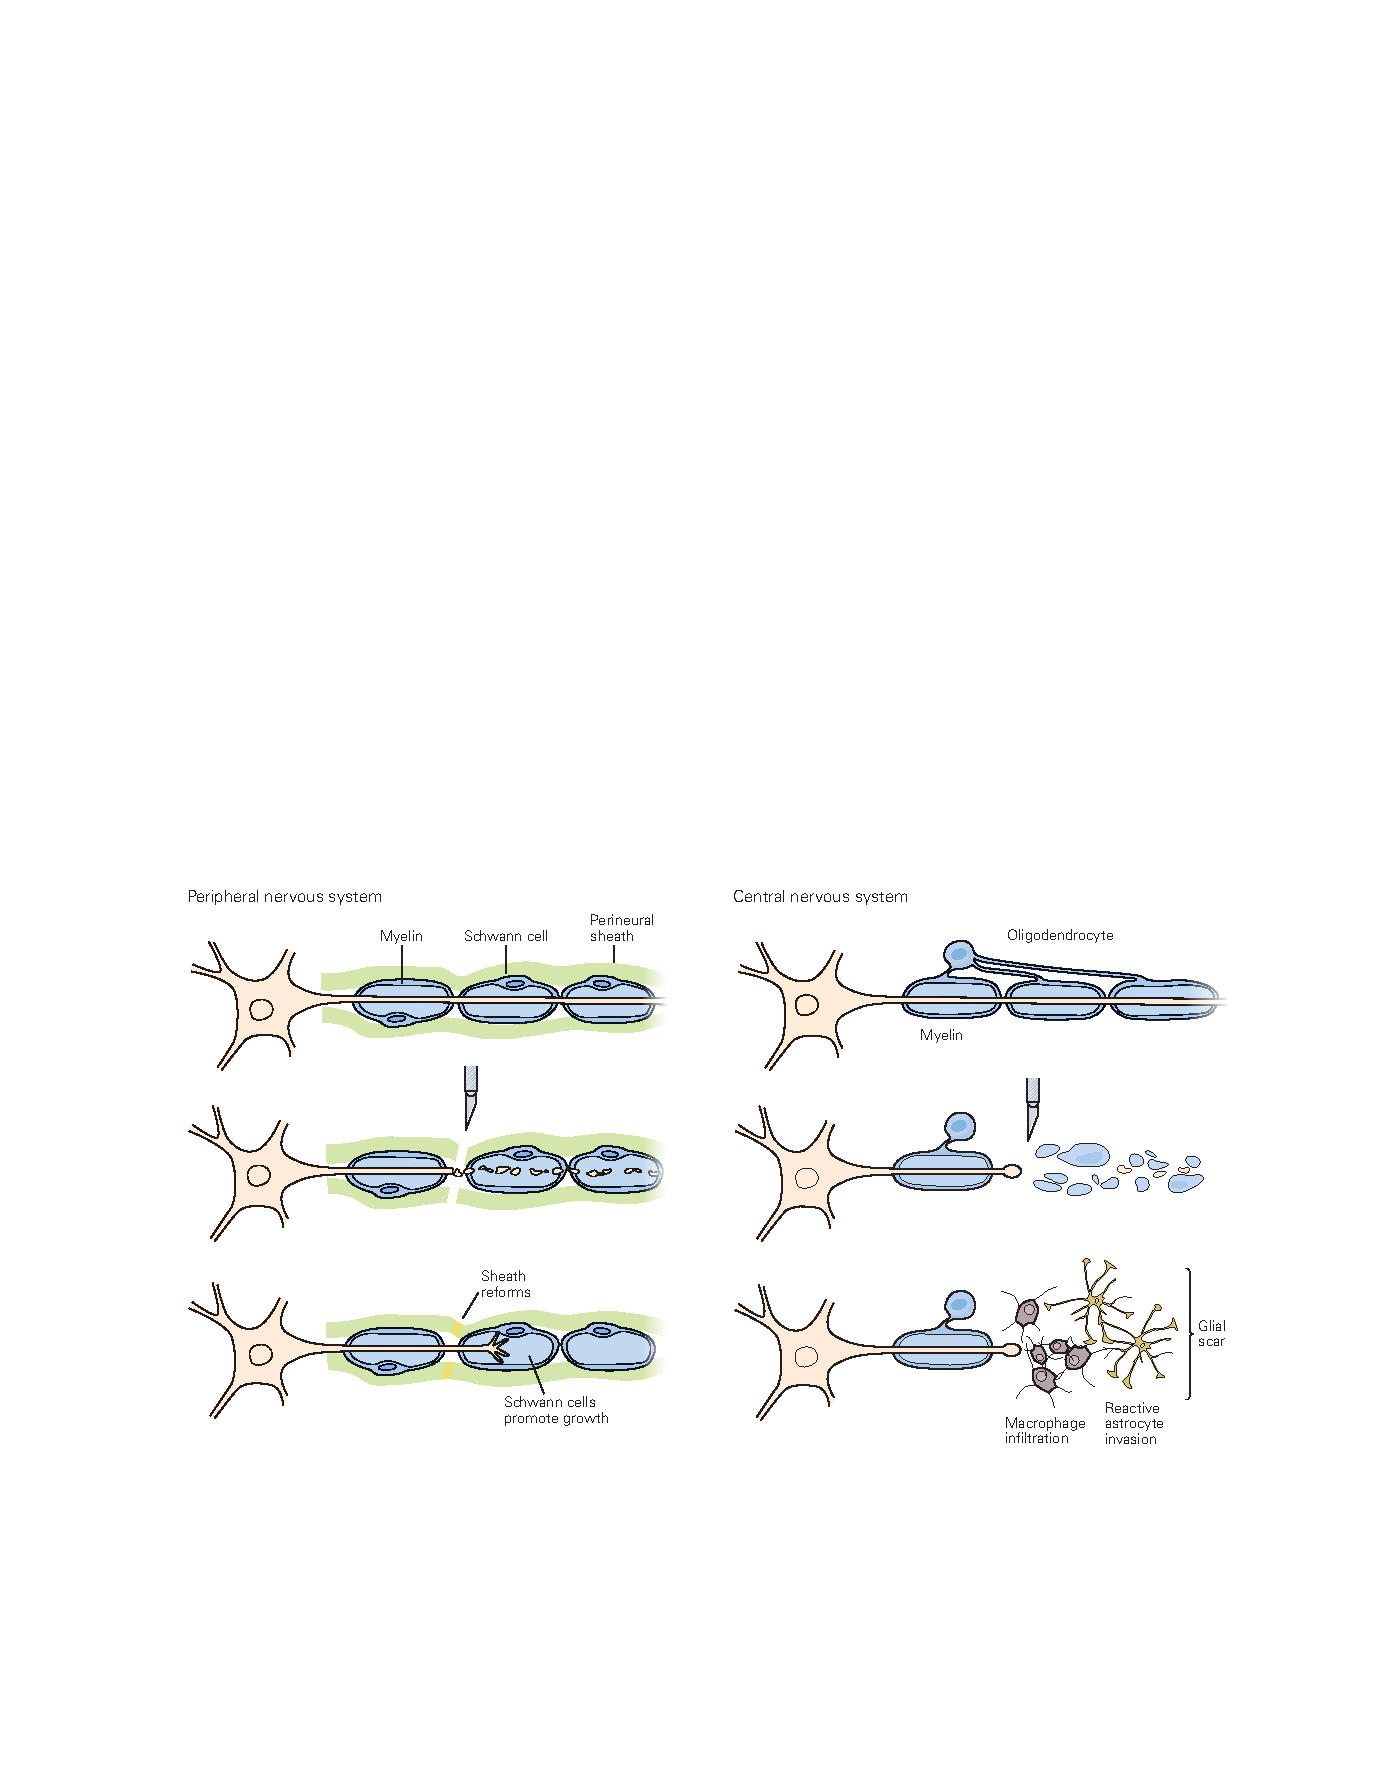
\includegraphics[width=1.0\linewidth]{chap50/fig_50_4}
	\caption{周围的轴突比中枢神经系统的轴突再生得更好。
		周围神经切片后,神经鞘迅速重塑,远端残端的雪旺氏细胞通过产生营养因子和引诱因子并表达高水平的粘附蛋白来促进轴突生长。
		在中枢神经系统轴突切片后,远端部分分解,髓鞘碎片。
		此外,反应性星形胶质细胞和巨噬细胞被吸引到病变部位。
		这种复杂的细胞环境,称为神经胶质疤痕,抑制轴突再生。}
	\label{fig:50_4}
\end{figure}


一旦再生的外周轴突到达它们的目标,它们就能够形成新的功能性神经末梢。
运动轴突形成新的神经肌肉接头;
自主神经轴突成功地重新支配腺体、血管和内脏;
和感觉轴突重新支配肌梭。
最后,那些失去髓鞘的轴突被重新髓鞘化,并且色谱细胞体恢复了原来的外观。
因此,在周围神经系统的所有三个部分(运动、感觉和自主),轴突切断术的影响是可逆的。
然而,外围再生并不完美。
在运动系统中,力量的恢复可能很大,但精细动作的恢复通常会受损。
一些运动轴突永远找不到它们的目标,一些在不合适的肌肉上形成突触,一些运动神经元死亡。
然而,周围神经系统的再生能力令人印象深刻。


相比之下,中枢神经系统受伤后的再生能力较弱(图~\ref{fig:50_4})。
受损轴突的近端残端可以形成短芽,但这些短芽很快就会停滞并形成肿胀的末端,称为“回缩球”,无法继续生长。
远距离再生很少见。
中枢再生的失败导致人们长期相信大脑和脊髓的损伤在很大程度上是不可逆的,治疗必须仅限于康复措施。


一段时间以来,神经生物学家一直在寻找中枢神经系统和周围神经系统的再生能力差异如此巨大的原因。
这项工作的目标是确定再生的关键障碍,以便克服这些障碍。
这些研究已经开始取得成果,现在人们谨慎乐观地认为,受伤的人类大脑和脊髓具有最终可以被利用的再生能力。


在讨论这些新发展之前,在更广泛的生物学背景下考虑神经再生问题是有帮助的。
是外周轴突的再生能力不寻常,还是中央轴突不能再生? 
事实上是后者。
显然,中央轴突在发育过程中生长良好。
更令人惊讶的是,未成熟哺乳动物的轴突也可以在大脑或脊髓横断后再生。
此外,鱼和青蛙等低等脊椎动物的成年中枢神经系统的再生能力很强,\textit{罗杰$\cdot$斯佩里}对视神经损伤后视力恢复的研究就是一个例证(第~\ref{chap:chap47}~章)。


那么为什么成熟的哺乳动物会失去这种看似重要的修复能力呢?
答案可能就在于哺乳动物的大脑有什么绝世之作,那就是在出生后早期的关键时期,根据经验重塑其基本线路图,使每个人的大脑得到优化,以应对内部和外部环境的变化和挑战。
外部世界(第~\ref{chap:chap49}~章)。
一旦发生重塑,就必须对其进行稳定。
如果另一只眼睛在儿童时期失明,虽然将皮层空间重新分配给一只眼睛显然是有用的,但我们不希望我们的皮层连接以类似的方式重新排列以响应短暂的不寻常的光照或黑暗。
因此,在面对连接性的小扰动时保持恒定可能会不可避免地导致限制中枢连接响应损伤而再生的能力。
从这个角度来看,我们有限的再生能力是一种浮士德式的交易,我们牺牲了恢复能力来确保维持作为我们卓越智力基础的精确连接回路。



\section{治疗干预可能促进受伤中枢神经元的再生}

在寻找中央轴突再生不良的原因时,一个关键问题是它是否反映了神经元自身无法生长或环境无法支持轴突生长。
\textit{阿尔伯特$\cdot$阿瓜约}和他的同事在 1980 年代初解决了这个问题。
他们将中枢神经干的片段插入周围神经,并将周围神经的片段插入大脑或脊髓,以了解轴突在面对新环境时会如何反应。


正如预期的那样,从胞体中分离出来的移植物中的轴突迅速退化,留下含有胶质细胞、支持细胞和细胞外基质的“远端残端”。
引人注目的是易位区段附近轴突的行为。
脊髓损伤后再生不良的脊髓轴突长入外周移植物数厘米(图~\ref{fig:50_5})。
同样,在视神经受损后再生不良的视网膜轴突会长到很长的距离,进入放置在其路径上的外周移植物。
相反,外周轴突通过其自身的远端神经干再生良好,但与切断的视神经配对时表现不佳(图~\ref{fig:50_6})。


\begin{figure}[htbp]
	\centering
	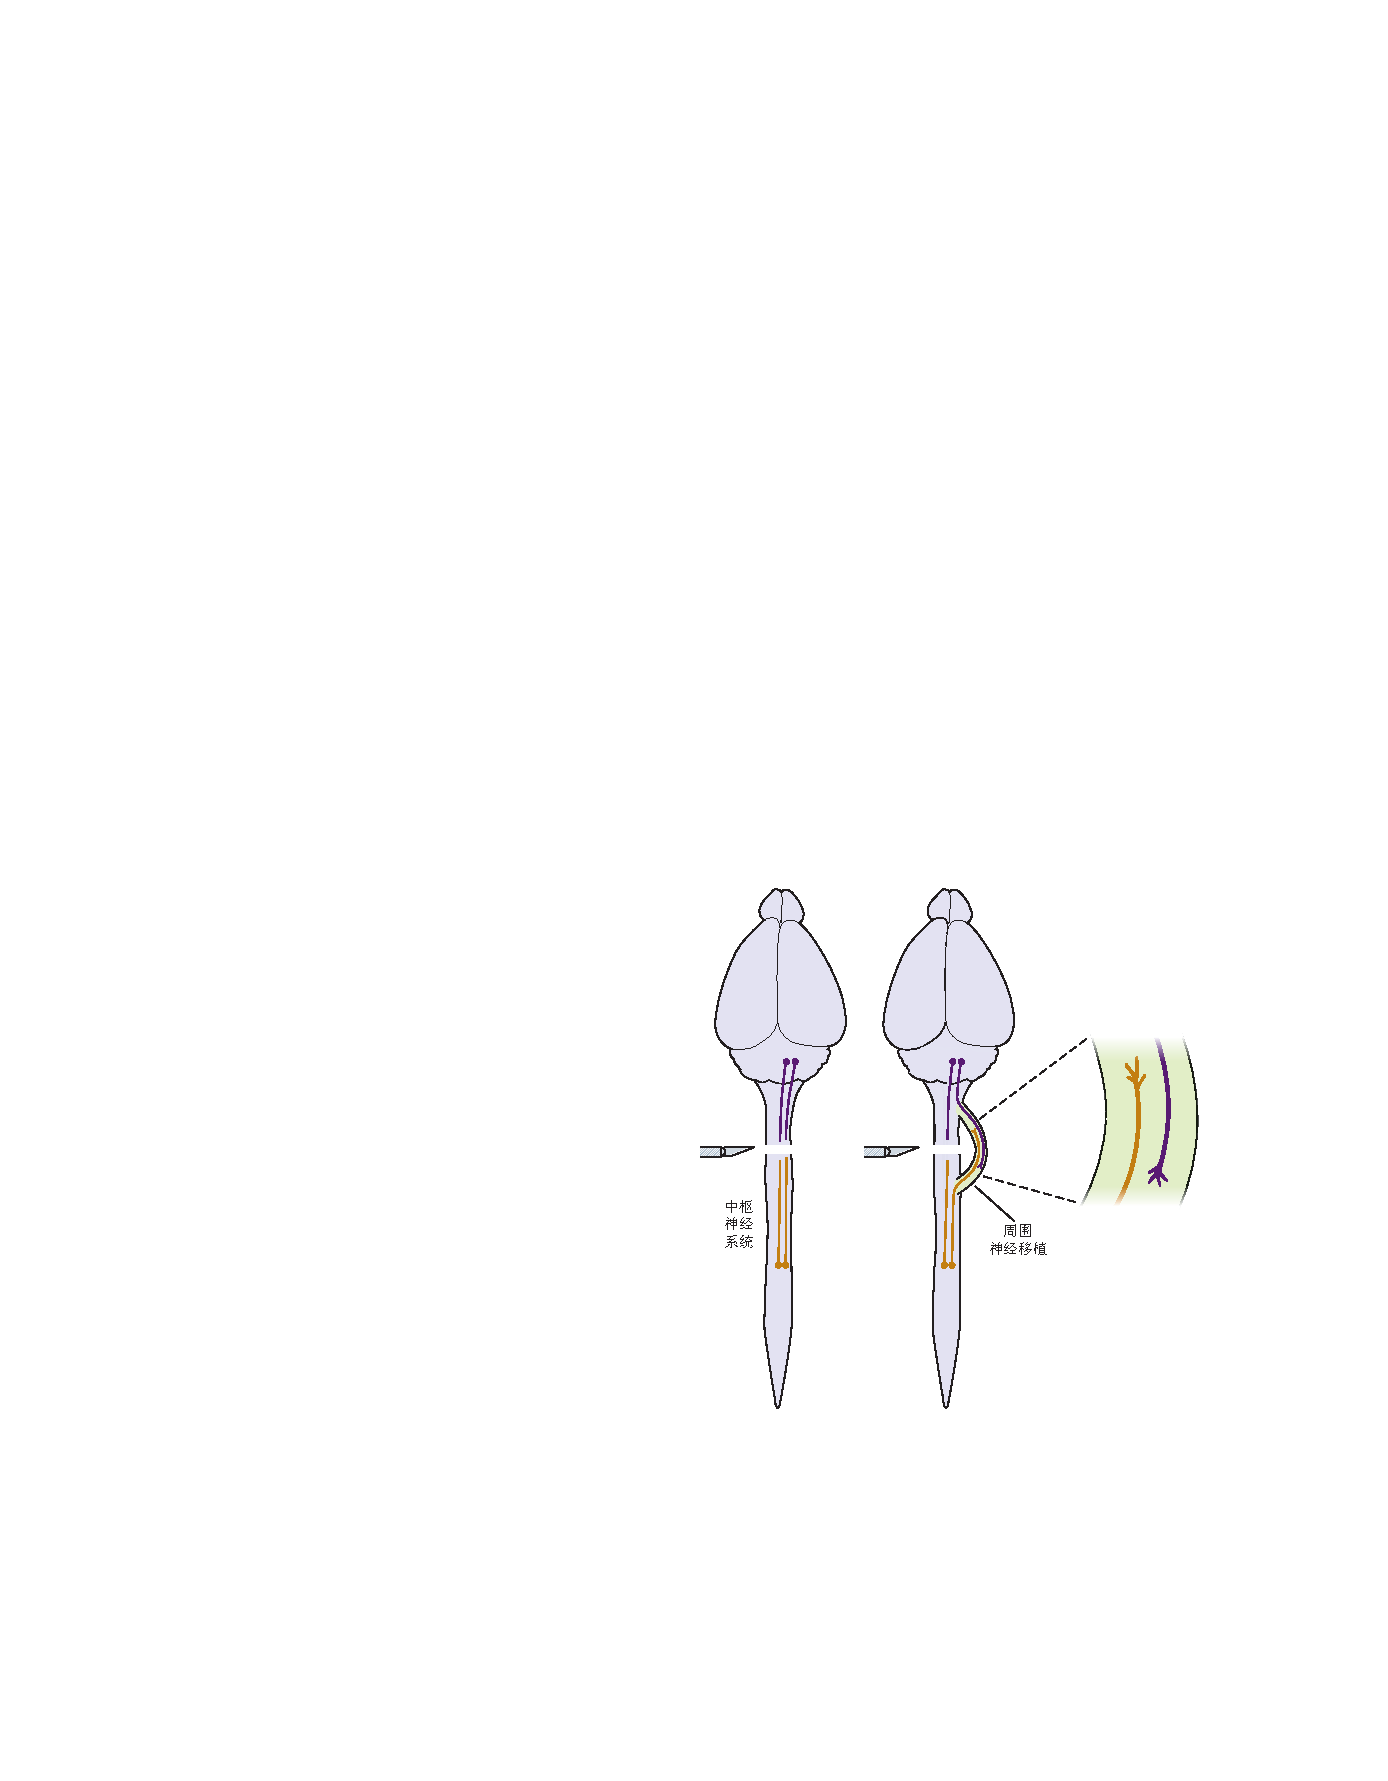
\includegraphics[width=0.65\linewidth]{chap50/fig_50_5}
	\caption{移植的周围神经为中枢轴突的再生提供了有利的环境。
		左图:脊髓切片后,上升和下降轴突无法穿过病变部位。
		右图:插入绕过损伤部位的周围神经移植物可促进上升轴突和下降轴突的再生\cite{david1981axonal}。}
	\label{fig:50_5}
\end{figure}


\begin{figure}[htbp]
	\centering
	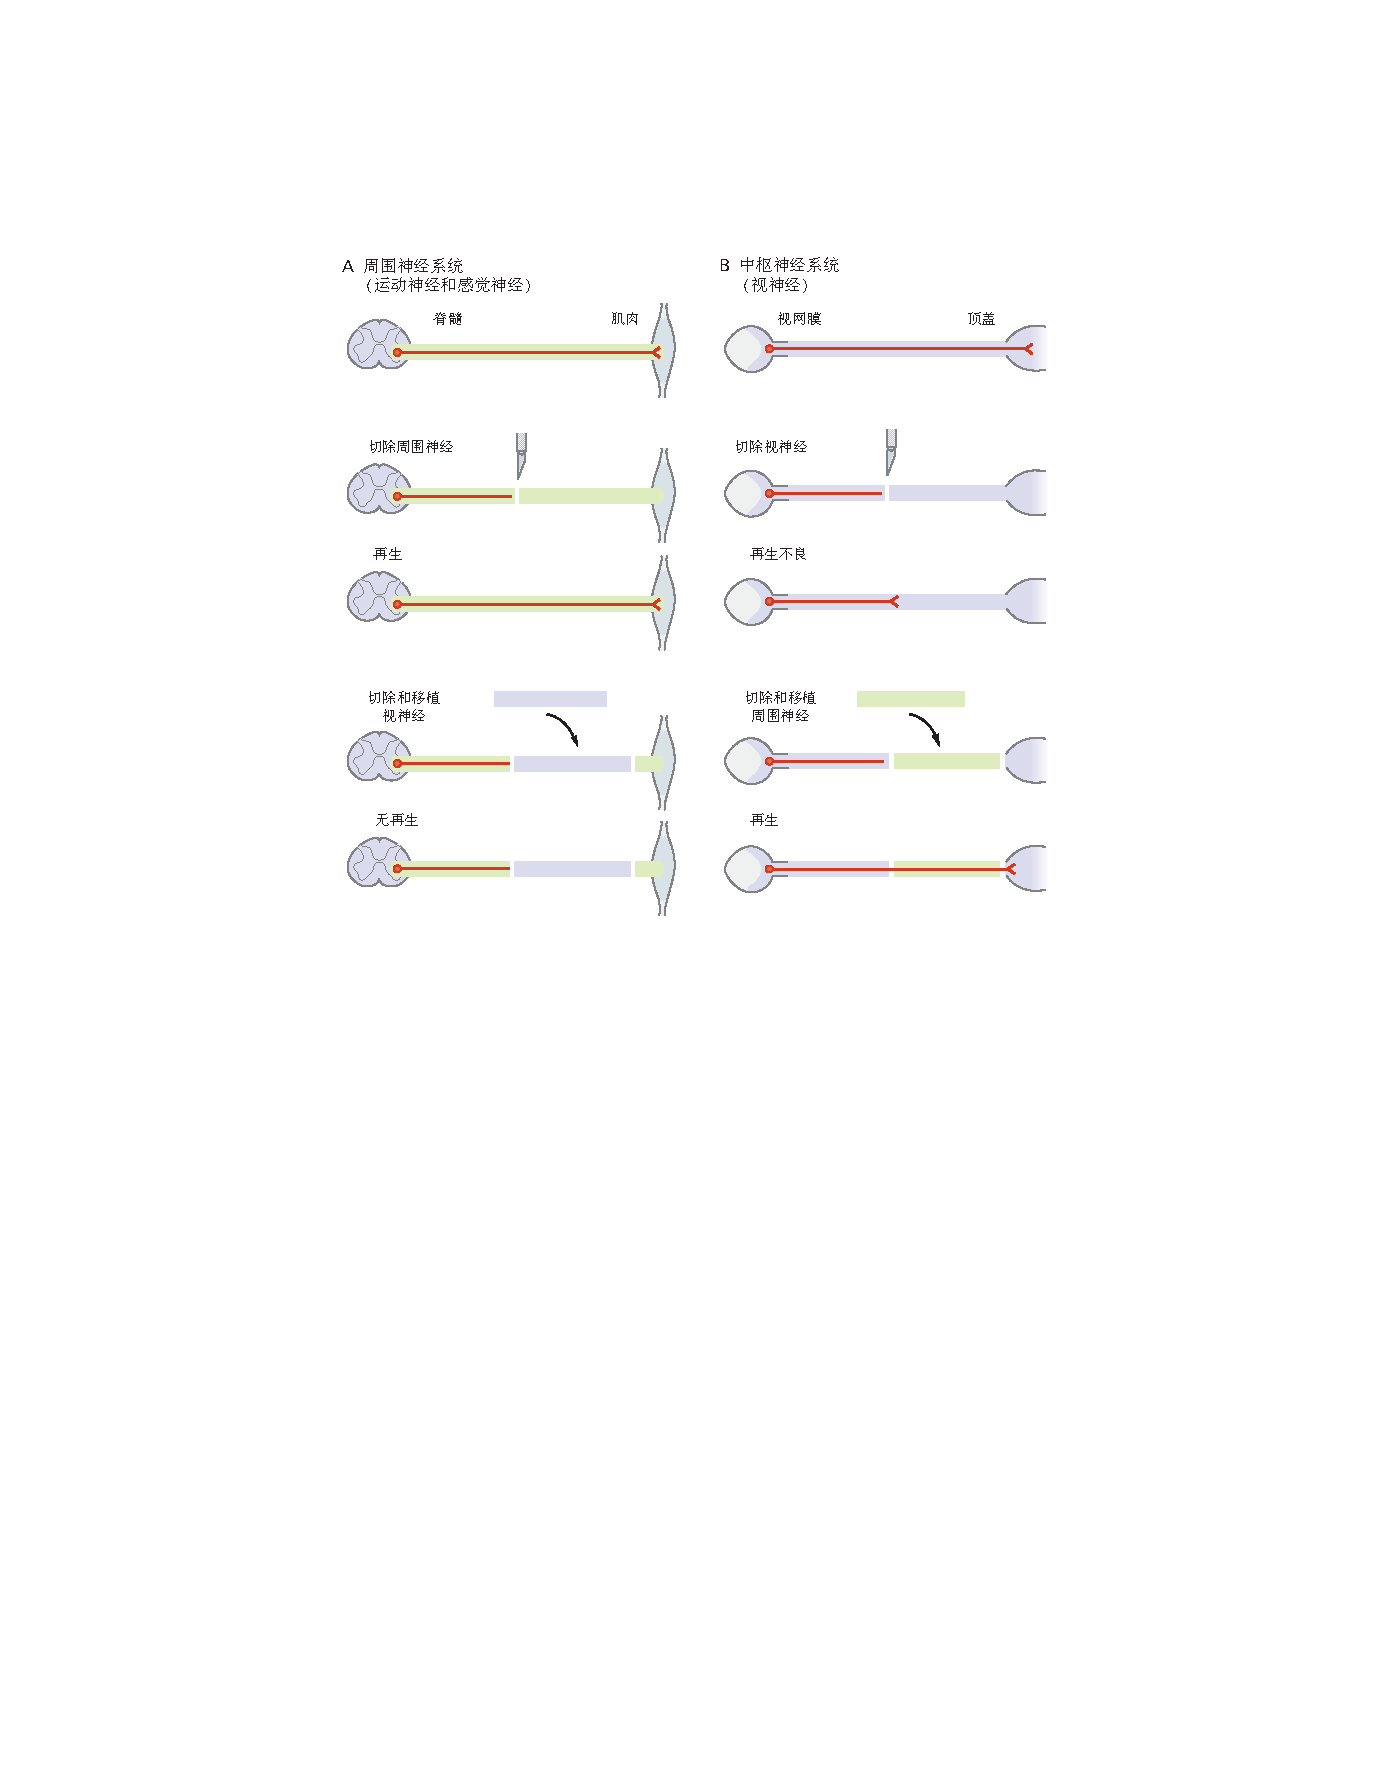
\includegraphics[width=0.89\linewidth]{chap50/fig_50_6}
	\caption{外周神经和中枢神经支持轴突再生的能力不同。
		\textbf{A.} 在周围神经系统中,被切断的轴突会在受伤部位重新长出。
		将一段视神经插入周围神经会抑制周围神经再生的能力。
		\textbf{B.} 在中枢神经系统中,被切断的轴突通常无法通过受伤部位重新生长。
		将一段周围神经插入中枢神经束可促进再生。}
	\label{fig:50_6}
\end{figure}


\textit{阿瓜约}扩展了这些研究,表明来自多个区域的轴突,包括嗅球、脑干和中脑,如果提供合适的环境,都可以长距离再生。
由于我们将在后面的部分讨论的原因,即使是最佳环境也不能完全恢复中央轴突的生长潜力。
尽管如此,这些开创性的实验将注意力集中在抑制再生能力的中央环境成分上,并促使人们深入寻找罪魁祸首。



\subsection{环境因素支持受伤轴突的再生}

在探索外围和中心生长环境之间的差异时,最初的搜索受到了 \textit{拉蒙-卡哈尔}的学生\textit{弗朗西斯科$\cdot$特略}进行的实验结果的影响,比\textit{阿瓜约}的研究早了将近一个世纪。
\textit{特略}将周围神经的片段移植到实验动物的大脑中,发现受伤的中央轴突向植入物生长,而当没有植入物时,它们几乎不生长。


这一结果表明外周细胞为受伤区域提供了生长促进因子,而这些因子在大脑中通常是不存在的。
\textit{拉蒙-卡哈尔}推断,中枢神经通路缺乏“能够维持和促进惰性和稀疏生长的物质”,类似于外周通路所提供的物质。
在接下来的一个世纪里,大量研究确定了周围神经的成分是神经突长出的有效促进剂。
这些包括雪旺细胞基底层的成分,例如层粘连蛋白和免疫球蛋白超家族的细胞粘附分子。
此外,去神经的远端神经残端中的细胞开始产生第~\ref{chap:chap46}~章中描述的神经营养蛋白和其他营养分子。
这些分子共同滋养神经元并引导胚胎神经系统中轴突的生长,因此它们也促进 轴突的再生。
相比之下,中枢神经元组织是这些分子的贫乏来源,含有少量层粘连蛋白和低水平的营养分子。
因此,在胚胎中,中枢和周围神经系统都提供了促进轴突生长的环境。
但只有外围环境才能在成年期保留这种能力,或者能够在受伤后有效地恢复这种能力。


这种观点的实际意义是,用促进生长的分子补充中央环境可能会改善再生。
为此,研究人员将神经营养蛋白注入损伤区域或插入富含细胞外基质分子(如层粘连蛋白)的纤维,作为轴突生长的支架。
在一些尝试中,雪旺细胞本身,或经过工程改造可分泌营养因子的细胞,已被移植到损伤部位。
在许多这样的情况下,受伤的轴突比在控制条件下生长得更广泛。
然而,再生仍然有限,轴突通常无法延伸很远的距离。
更重要的是,功能恢复很少。



\subsection{髓磷脂的成分抑制神经突生长}

是什么导致如此有限的再生?
部分解释是,被切断的中央轴突所处的环境不仅缺乏生长促进因子,而且富含生长抑制因子,其中一些来自髓鞘。
在培养中,中枢而非外周髓鞘的片段有效地抑制了共培养的中枢或外周神经元的神经突生长。
相反,在经过治疗以防止脊髓中髓磷脂形成的大鼠中,损伤后脊髓轴突侧枝的发芽得到增强(图~\ref{fig:50_7})。


\begin{figure}[htbp]
	\centering
	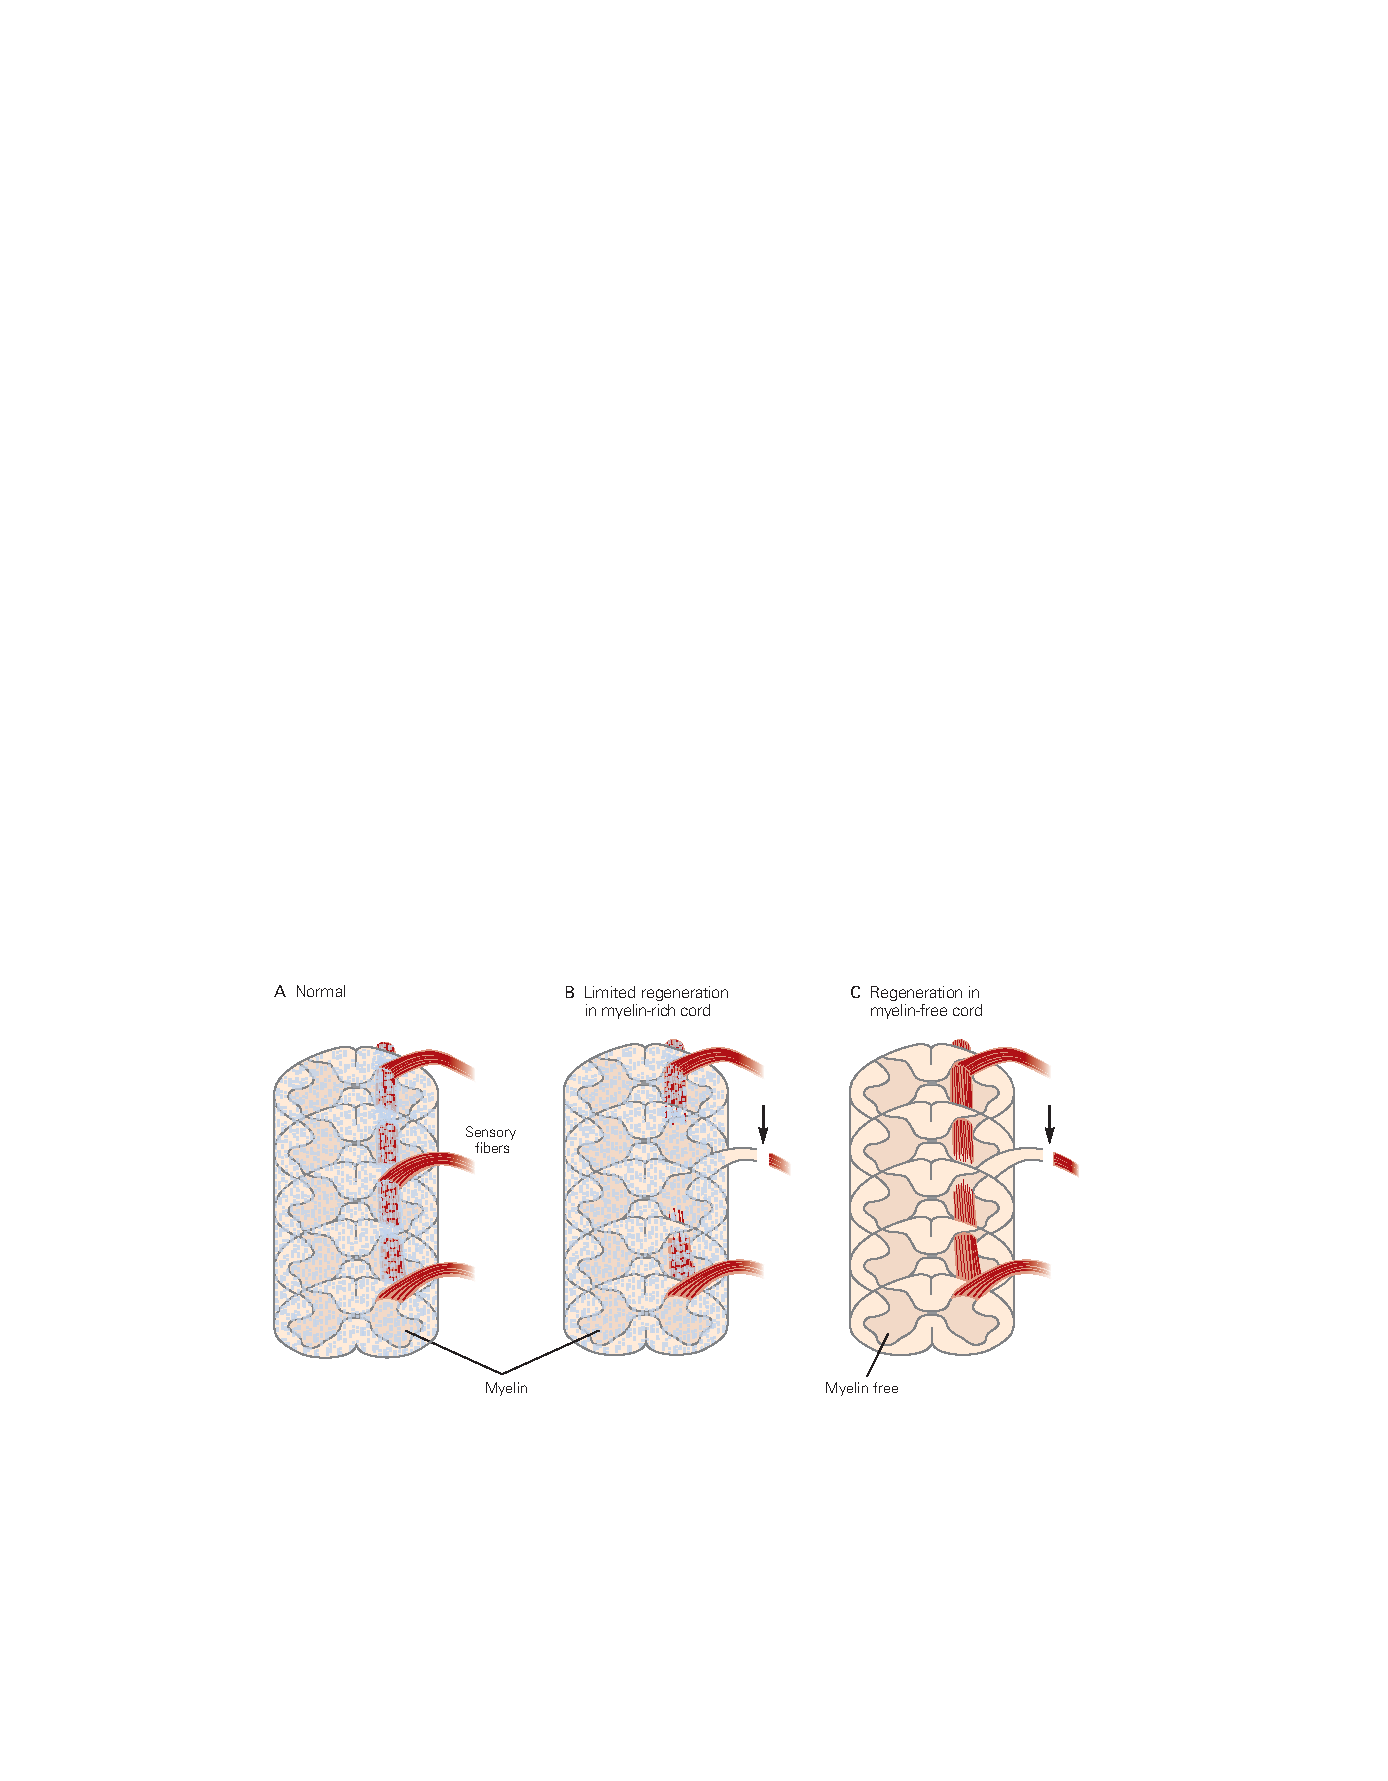
\includegraphics[width=0.9\linewidth]{chap50/fig_50_7}
	\caption{髓磷脂抑制中央轴突的再生\cite{schwegler1995increased}。
		\textbf{A.} 感觉纤维通常在富含髓磷脂的脊髓中向头端延伸。
		\textbf{B.} 右背根纤维在 2 周大的正常大鼠中切片。
		20 天后对纤维的再生进行组织化学评估。
		被切开的轴突的中央分支退化,使一部分脊髓失去神经支配。
		富含髓磷脂的脐带几乎没有再生。
		\textbf{C.} 一些同窝仔接受局部 X 射线照射以阻断髓鞘形成。
		在这些动物中,通过邻近未受伤的根部进入脐带的感觉纤维在去神经支配后长出了新的侧枝。}
	\label{fig:50_7}
\end{figure}


这些发现表明,尽管中枢和外周环境都可能含有促进生长的元素,但中枢神经也含有抑制成分。
髓鞘抑制神经突生长的事实可能看起来很奇怪,但如果我们考虑到髓鞘形成通常发生在出生后,即轴突延伸基本完成之后,就不是这样了。


寻找中枢髓磷脂的抑制成分发现了一大堆难题。
与外周髓磷脂相比,中央髓磷脂中出现的几类分子在呈现给培养的神经元时能够抑制神经突生长。
当针对髓磷脂蛋白产生的抗体被证明能够部分中和髓磷脂抑制神经突长出的能力时,发现了第一个发现。
使用这种抗体分离相应的抗原产生了现在称为 Nogo 的蛋白质。
另外两种蛋白质,\textit{髓磷脂相关糖蛋白}和\textit{髓鞘少突胶质细胞糖蛋白},最初作为髓鞘的主要成分被分离出来,也被发现可以抑制某些神经元类型的生长。


有趣的是,Nogo、\textit{髓磷脂相关糖蛋白}和\textit{髓鞘少突胶质细胞糖蛋白}与常见的膜受体 NogoR 和 PirB 结合(图~\ref{fig:50_8})。
NogoR 以及与生长抑制有关的相关受体,如 LINGO,都与神经营养蛋白受体 p75 相互作用(第~\ref{chap:chap46}~章)。
这种相互作用将 p75 从促进生长的受体转变为抑制生长的受体。
也许是因为有太多的生长抑制因子和受体,在缺少其中任何一种的突变小鼠中,中央轴突的再生并没有大大增强。
然而,许多抑制成分会触发激活 RhoA 的相同细胞内信号通路,从而刺激 Rho 激酶(ROCK);
ROCK 反过来导致生长锥坍塌并阻断神经突生长所需的肌动蛋白和微管蛋白聚合。
目前的研究正在探索干扰该共享通路是否可以一次性抵消许多抑制剂的影响。


\begin{figure}[htbp]
	\centering
	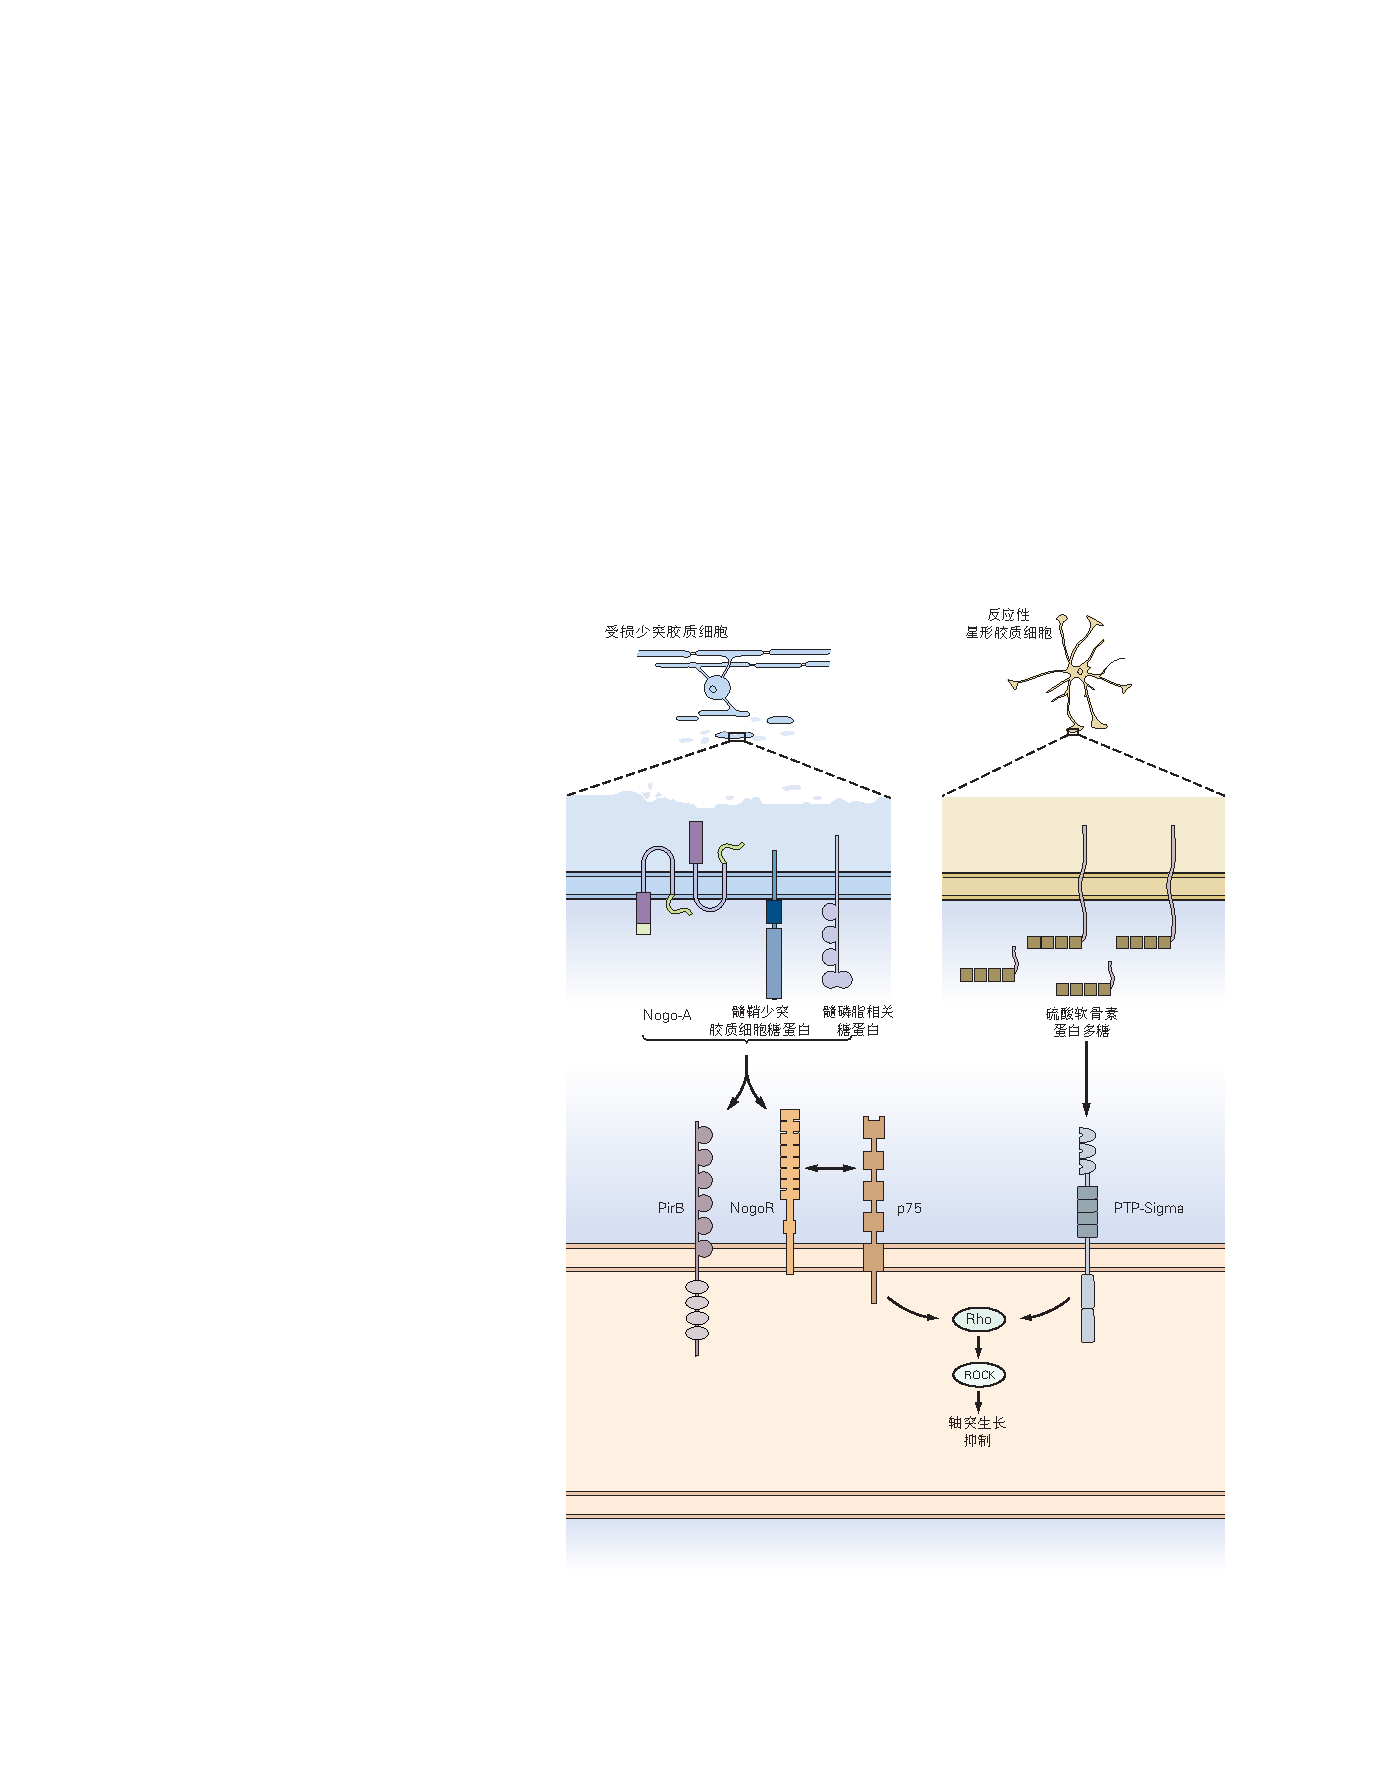
\includegraphics[width=0.85\linewidth]{chap50/fig_50_8}
	\caption{抑制中央轴突再生的髓磷脂和神经胶质疤痕成分\cite{yiu2006glial}。
		左图:髓磷脂含有蛋白质 Nogo-A、\textit{髓鞘少突胶质细胞糖蛋白}和\textit{髓磷脂相关糖蛋白}。
		当髓磷脂分解时,所有三种蛋白质都会暴露出来。
		它们可以结合受体蛋白 NogoR,后者可以与神经营养蛋白受体 p75 以及免疫球蛋白样受体蛋白 PirB 结合。
		PirB 的失活导致皮层脊髓轴突再生的适度增强。
		右图:\textit{硫酸软骨素蛋白多糖}是胶质瘢痕的主要成分,被认为通过与受体酪氨酸磷酸酶 PTP-sigma 相互作用来抑制轴突再生,PTP-sigma 激活细胞内介质,如 Rho 和 ROCK。}
	\label{fig:50_8}
\end{figure}



\subsection{损伤引起的疤痕阻碍轴突再生}

髓鞘碎片并不是受伤大脑或脊髓中生长抑制物质的唯一来源。
如前所述,星形胶质细胞在受伤后被激活并增殖,获得在受伤部位产生疤痕组织的反应性星形胶质细胞的特征。
疤痕形成是一种适应性反应,有助于限制损伤的大小、重建血脑屏障并减少炎症。


但疤痕本身以两种方式阻碍再生:
通过机械干扰轴突生长和通过疤痕内细胞产生的蛋白质的生长抑制作用。
这些抑制剂中最主要的是一类\textit{硫酸软骨素蛋白多糖},它由反应性星形胶质细胞大量产生,并通过与轴突上的酪氨酸磷酸酶受体相互作用直接抑制轴突延伸(图~\ref{fig:50_8})。
因此,注意力集中在通过注入一种叫做软骨素酶的酶来溶解神经胶质疤痕的方法,这种酶可以分解\textit{硫酸软骨素蛋白多糖}上的糖链。
这种治疗促进了动物的轴突再生和功能恢复。
减少炎症和减少疤痕形成的药物,特别是泼尼松龙,如果在受伤后不久、疤痕形成之前服用,也是有益的。



\subsection{内在增长计划促进再生}

到目前为止,我们已经强调了外周轴突和中央轴突的局部环境之间的差异。
然而,环境差异不能完全解释中央轴突再生不良的原因。
尽管它们可以在外周神经中再生,但在沿着相同路径行驶时,中枢轴突的生长情况远不如外周轴突。
因此,成人中央轴突的再生能力可能不如外周轴突。


为支持这一想法,组织培养实验表明,中枢神经元的生长潜力会随着年龄的增长而降低,而成熟的外周神经元在有利的环境中会稳健地延伸轴突。
对这种差异的一个可能解释是被认为对最佳轴突伸长至关重要的蛋白质表达的变化。
一个例子是 43 kDa 生长相关蛋白,或\textit{神经生长相关蛋白-43}。
这种蛋白质在胚胎中枢神经元和外周神经元中以高水平表达。
在外周神经元中,成熟度水平仍然很高,并且在轴突切开术后增加更多,而在中枢神经元中,其表达随着发育的进行而降低。
协调轴突生长程序所需的转录因子也在发育过程中以高水平表达,然后在成熟过程中下调。


中央轴突再生能力的降低是否可逆?
两组研究提供了希望。
其中之一涉及所谓的“条件性损伤”。
回想一下,背根神经节中的初级感觉神经元有一个分叉的轴突,一个外围分支延伸到皮肤、肌肉或其他目标,一个中央分支进入脊髓。
外围分支在受伤后再生良好,而中央分支再生较差。
然而,如果外围分支在中央分支受损前几天受损,中央分支将成功再生(图~\ref{fig:50_9})。
不知何故,先前的伤害或条件性损伤会激活轴突生长程序。


\begin{figure}[htbp]
	\centering
	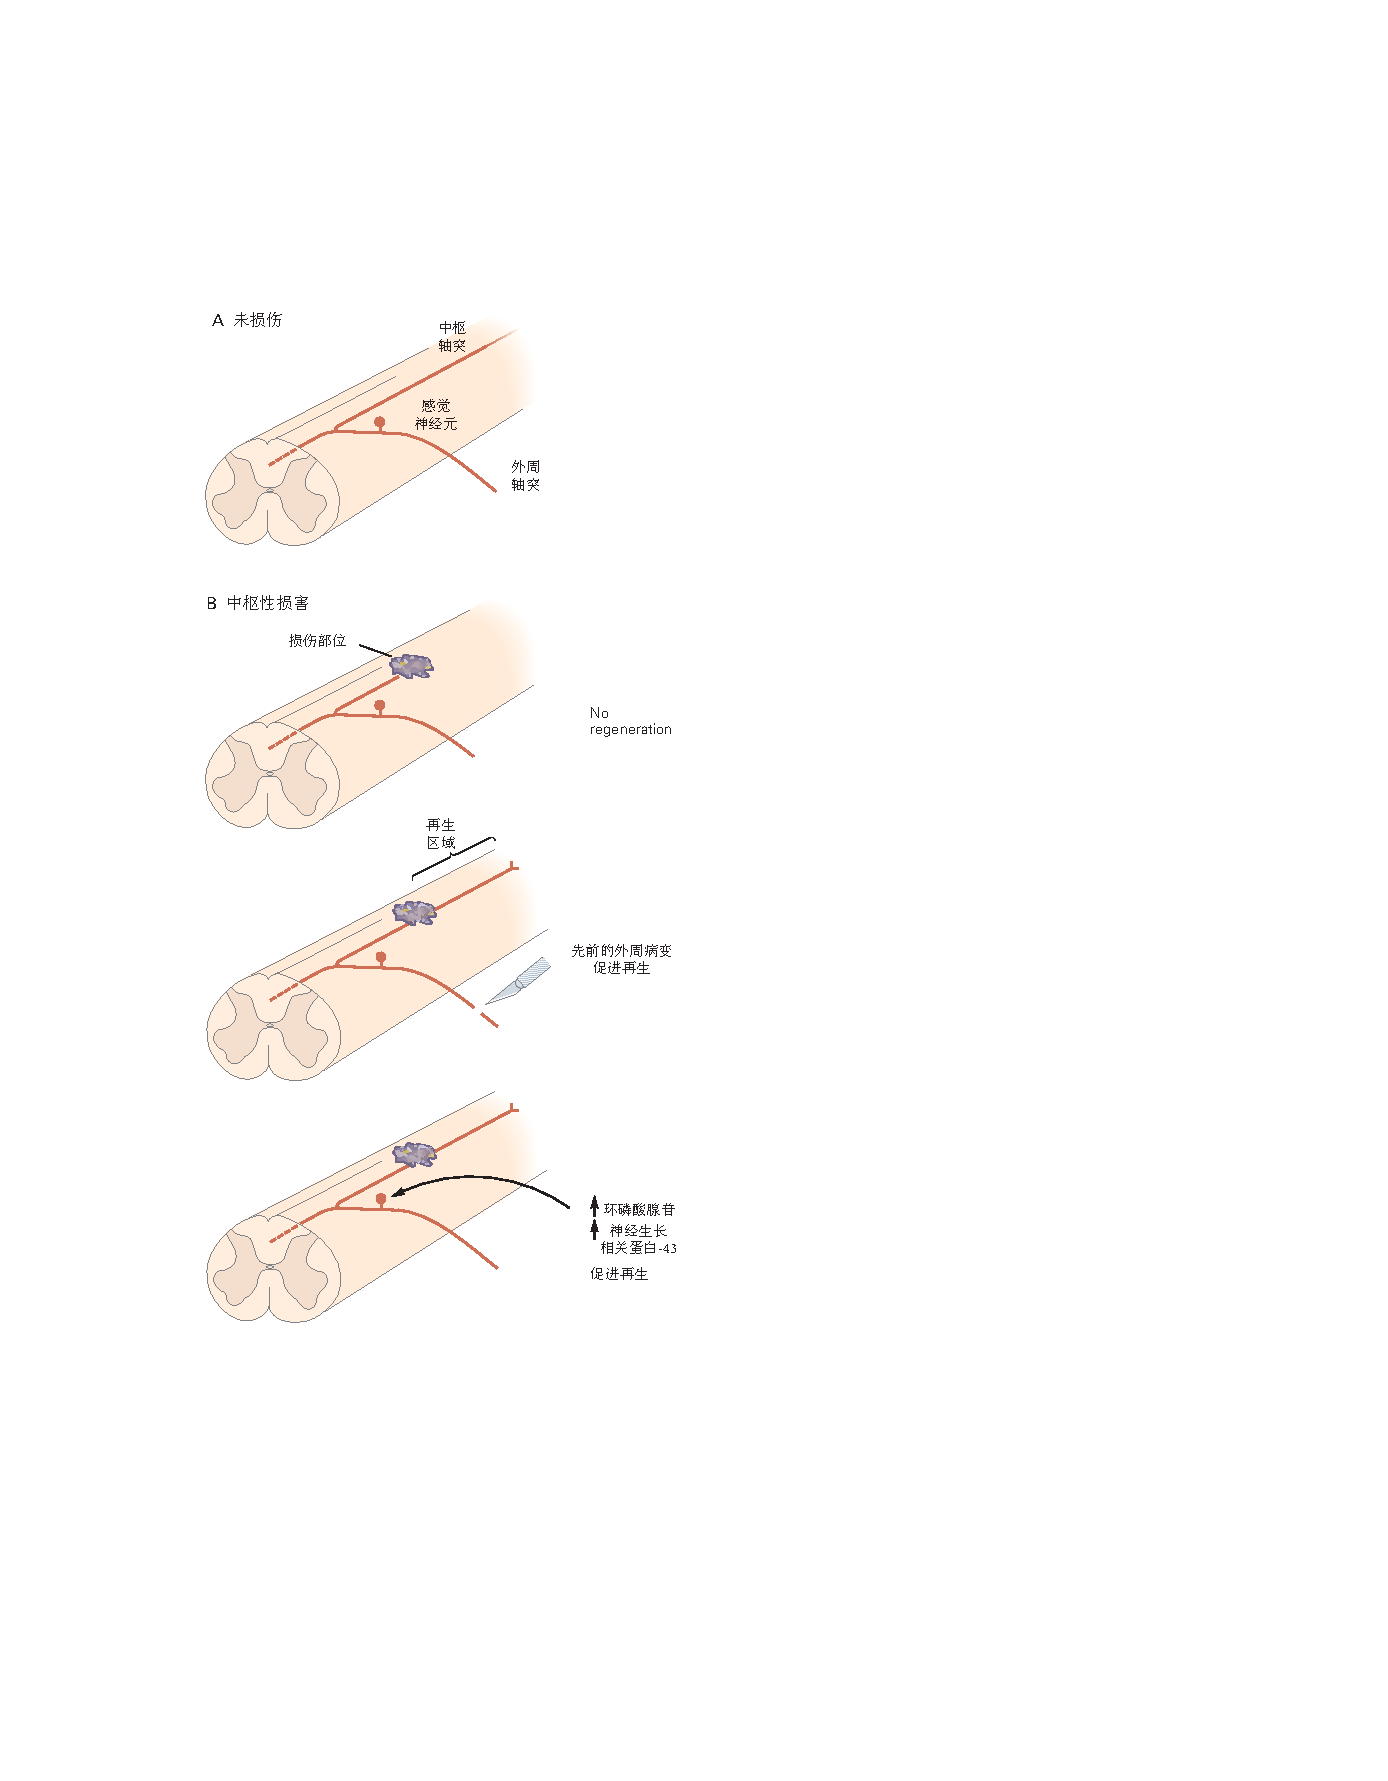
\includegraphics[width=0.65\linewidth]{chap50/fig_50_9}
	\caption{条件性损伤促进初级感觉神经元轴突中央分支的再生。
		脊髓损伤后,损伤部位以外的中央分支几乎没有再生。
		然而,如果轴突的外围分支在中央分支受损之前被切开,则后者会生长到病变部位之外。
		这种“条件性损伤”的影响可以通过提高周围分支中\textit{环磷酸腺苷}或生长相关蛋白\textit{神经生长相关蛋白-43}的水平来模拟。}
	\label{fig:50_9}
\end{figure}


负责中央分支再生的生长程序的一个组成部分似乎是\textit{环磷酸腺苷}。
这种第二信使分子激活酶,进而促进神经突生长。
当神经元最初形成回路时,\textit{环磷酸腺苷}的水平很高;
它们在中枢神经元而非外周神经元中在出生后下降。
在某些情况下,增加\textit{环磷酸腺苷}或通常由\textit{环磷酸腺苷}激活的蛋白质的供应可以促进损伤后中枢轴突的再生。
因此,增加\textit{环磷酸腺苷}水平或激活\textit{环磷酸腺苷}靶点的药物被积极考虑作为脊髓损伤后的治疗剂。


第二组研究操纵发育调节的内在因素来恢复成人的再生能力。
例如,损伤有时会导致\textit{睫状神经营养因子}等细胞因子的形成,这些细胞因子通过激活涉及称为 JAK 和 STAT 的分子的信号通路来促进生长,这些分子会进入细胞核并调节生长程序。
然而,在成人中,该通路被一种称为\textit{细胞因子信号通路抑制因子3}的蛋白质所抑制。
删除小鼠中的\textit{细胞因子信号通路抑制因子3}基因可解除抑制并增强细胞因子促进受损轴突再生的能力(图~\ref{fig:50_10}A)。


\begin{figure}[htbp]
	\centering
	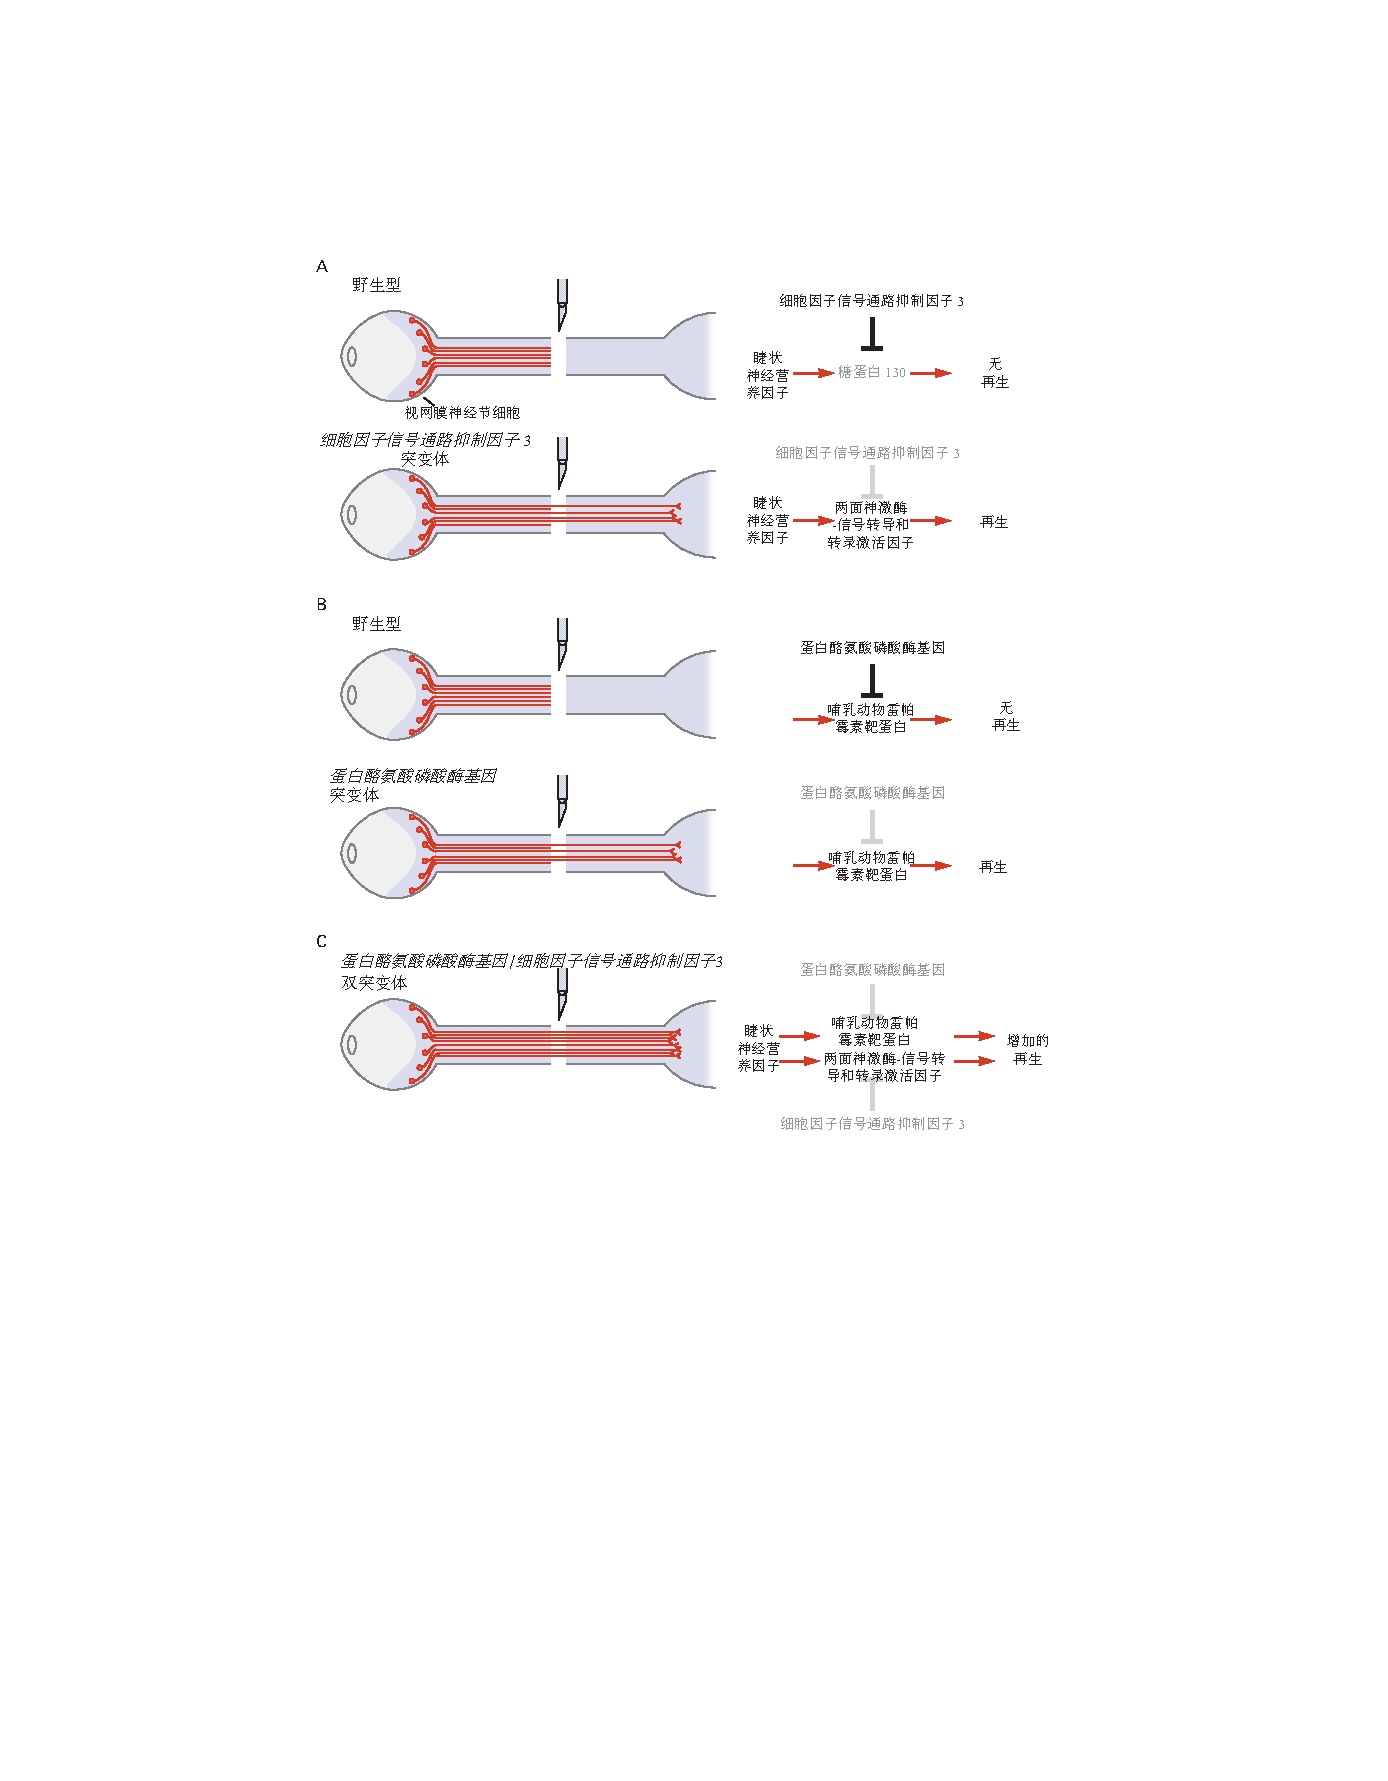
\includegraphics[width=0.76\linewidth]{chap50/fig_50_10}
	\caption{调节视神经轴突再生的信号通路。
		\textbf{A.} 视神经中视网膜神经节细胞轴突的再生通常受到几个基因的神经元表达的限制。
		一种编码\textit{细胞因子信号通路抑制因子3},它阻断\textit{睫状神经营养因子}结合其受体\textit{糖蛋白 130}的能力,从而阻断\textit{睫状神经营养因子}促进再生。
		在\textit{细胞因子信号通路抑制因子3}突变小鼠中,\textit{睫状神经营养因子}的环境水平足以改善视神经再生。
		消除\textit{糖蛋白 130}和\textit{细胞因子信号通路抑制因子3}会阻碍再生能力。
		添加额外的\textit{睫状神经营养因子}可增强\textit{细胞因子信号通路抑制因子3}突变小鼠的再生能力。
		\textbf{B.} 另一个基因编码\textit{蛋白酪氨酸磷酸酶基因},它通过调节能量代谢的\textit{哺乳动物雷帕霉素靶蛋白}通路阻断信号。
		因此,\textit{蛋白酪氨酸磷酸酶基因}突变小鼠的再生得到增强。
		\textbf{C.} 因为\textit{细胞因子信号通路抑制因子3}和\textit{蛋白酪氨酸磷酸酶基因}调节不同的生长促进信号,缺乏这两个基因的突变小鼠表现出比任何一个突变体更强的再生能力\cite{smith2009socs3}。}
	\label{fig:50_10}
\end{figure}


同样,涉及激酶\textit{哺乳动物雷帕霉素靶蛋白}的信号通路调节能量代谢,促进轴突再生所需的合成代谢生长促进状态。
然而,随着中枢神经元的成熟,\textit{哺乳动物雷帕霉素靶蛋白}被下调,并被称为\textit{蛋白酪氨酸磷酸酶基因}的磷酸酶进一步抑制。
类似于\textit{细胞因子信号通路抑制因子3}和\textit{两面神激酶-信号转导和转录激活因子}信号,小鼠中\textit{蛋白酪氨酸磷酸酶基因}基因的缺失促进了视神经或脊髓损伤后的轴突再生(图~\ref{fig:50_10}B)。
此外,\textit{细胞因子信号通路抑制因子3}和\textit{蛋白酪氨酸磷酸酶基因}的丢失比任何一个的丢失都更能刺激再生。
尽管它们的多重作用使得\textit{细胞因子信号通路抑制因子3}或 \textit{蛋白酪氨酸磷酸酶基因}不太可能成为有用的治疗靶点,但它们调节的信号通路为设计可以增强再生的药物提供了多个起点。



\subsection{完整轴突形成新的连接可导致损伤后功能的恢复}

到目前为止,我们已经讨论了旨在增强受损中枢轴突有限再生能力的干预措施。
另一种策略侧重于即使没有明显的切割轴突再生也能在受伤后发生的重要但不完全的功能恢复。
如果能够理解这种功能有限恢复的基础,就有可能加强它。


为应对损伤而重新排列现有的连接可能有助于功能的恢复。
我们已经了解到,轴突切开术会导致受损神经元的输入和目标发生变化。
尽管其中许多变化对功能有害,但有些变化是有益的。
特别是,中枢神经系统在受伤后可以自发地进行适应性重组,帮助其恢复功能。
例如,许多脊髓外伤都会发生下行皮层脊髓通路横断后,皮层不能再向损伤部位下方的运动神经元传递指令。
然而,在数周后,位于病变头端的完整皮层脊髓轴突开始长出新的末端分支,并在其轴突围绕病变延伸的脊髓中间神经元上形成突触,从而形成有助于有限恢复功能的脊柱内迂回(图~\ref{fig:50_11}) 。



\begin{figure}[htbp]
	\centering
	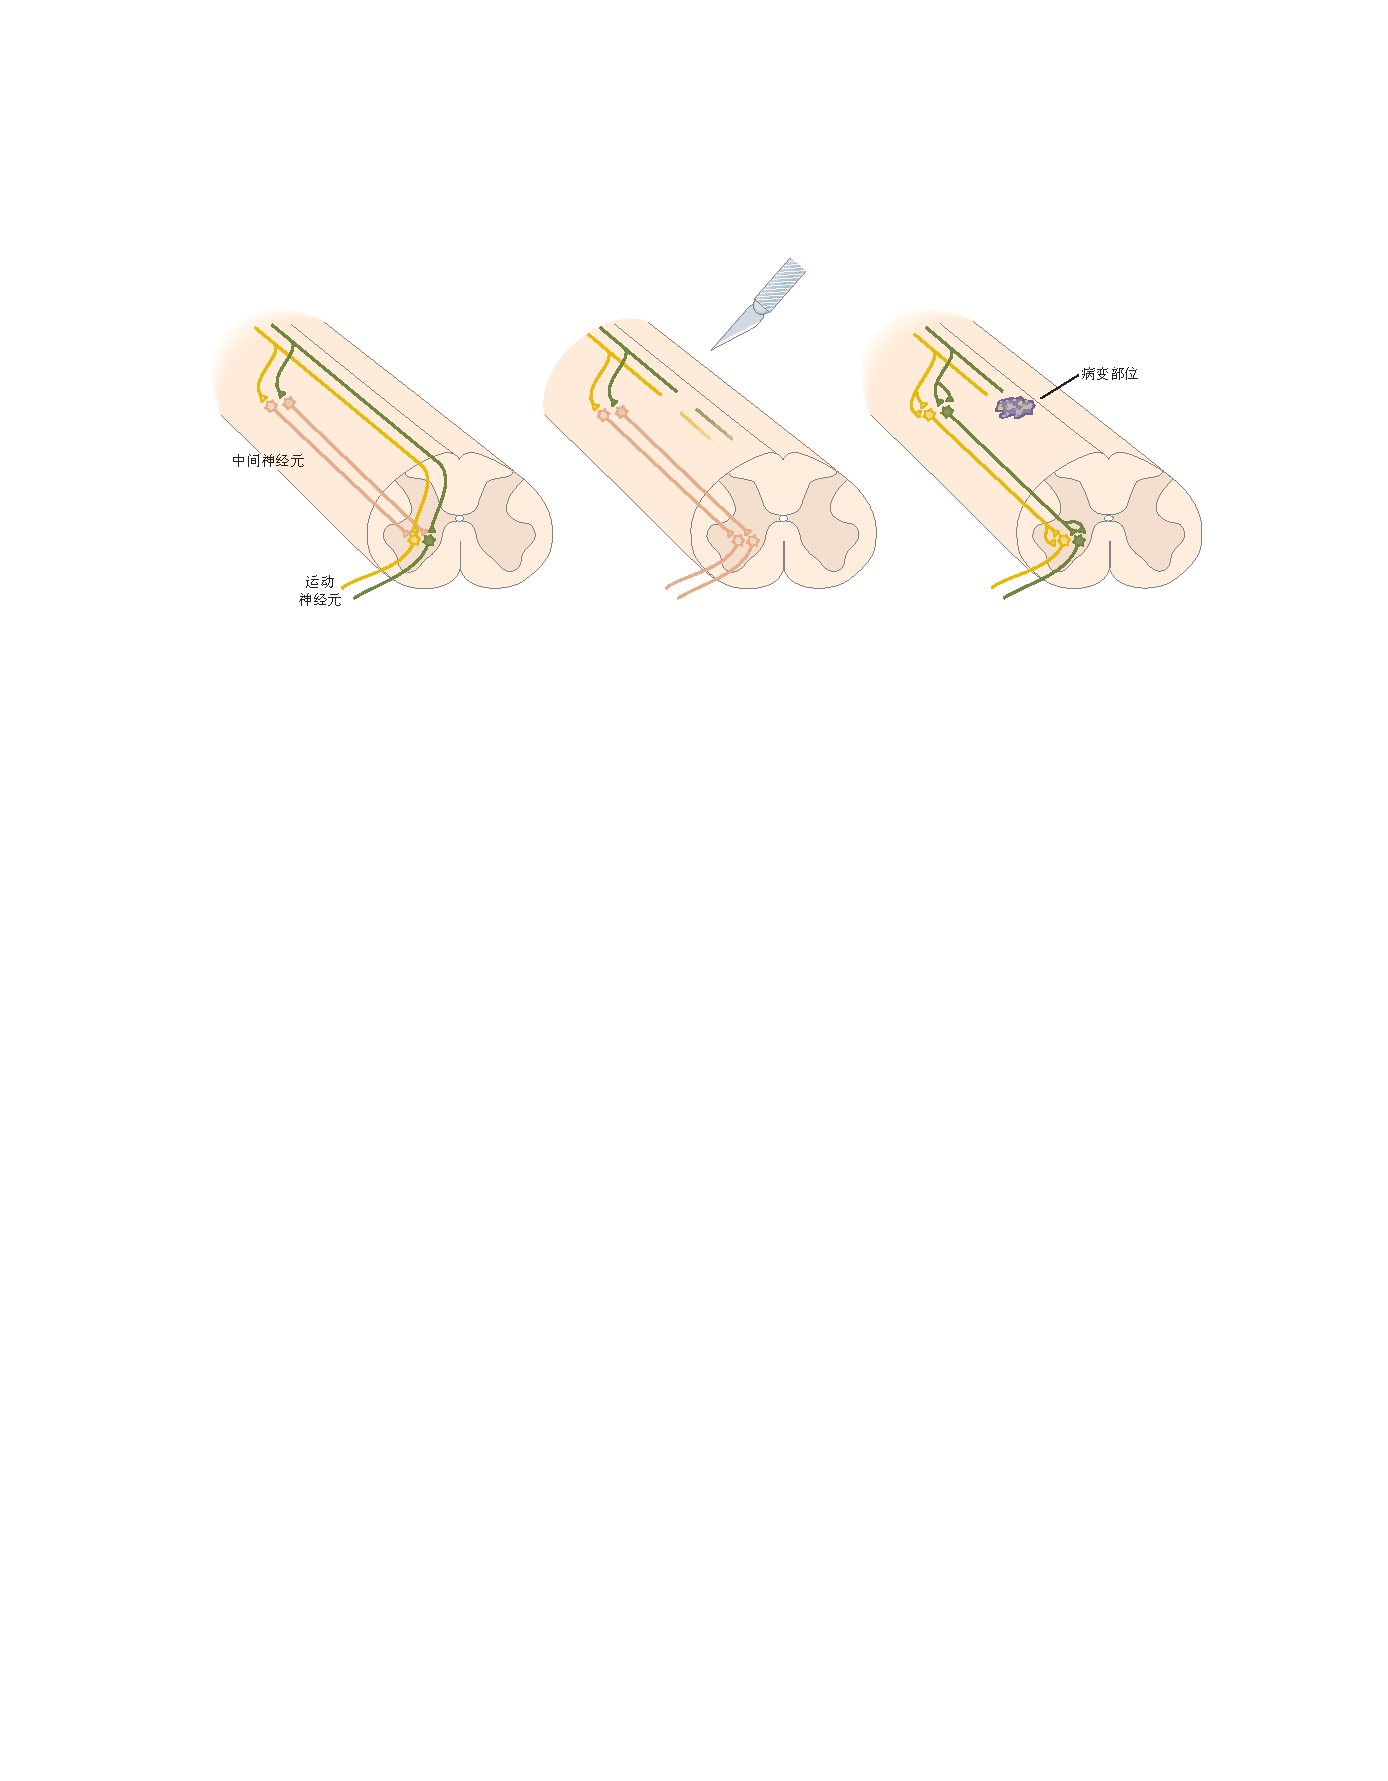
\includegraphics[width=1.0\linewidth]{chap50/fig_50_11}
	\caption{脊髓损伤后可以通过重组脊髓回路恢复功能。
		切断的皮层脊髓轴突可以通过发芽轴突侧枝来重新建立与运动神经元的连接,轴突侧枝支配神经元中间神经元,其轴突绕过病变并接触位于病变部位尾部的运动神经元\cite{bareyre2004injured}。}
	\label{fig:50_11}
\end{figure}


类似的功能重组实例已在运动皮层和脑干中得到证实。
这些补偿反应证明了神经系统的潜在可塑性。
神经系统重新连接自身的能力在出生后早期的关键时期最为活跃,但在成年期的创伤事件中可以恢复(第~\ref{chap:chap49}~章)。


如何提高中枢神经系统的重布线能力?
移植物对实验动物的一些有益影响可能反映了完整轴突的重组,而不是横断轴突的再生。
随着神经系统的可塑性得到更好的理解,促进回路特定变化的治疗策略可能成为可能。
也许最有前途的是一种方法,其中促进生长的细胞或分子干预与导致回路重新布线的行为疗法相结合。



\section{受伤大脑中的神经元死亡,但可以产生新的神经元}

无法长出新的轴突绝不是可能降临在受伤神经元身上的最糟糕的命运。
对于许多神经元,轴突切开术会导致细胞死亡。
因此,改善损伤后恢复的努力需要考虑神经元的存活,而不仅仅是轴突的再生。
由于神经元死亡是其他神经损伤(例如中风和神经退行性疾病)的常见后果,因此保留或替换神经元的改进方法将具有广泛的用途。


损伤后细胞的丢失并不是神经系统独有的,尽管在其他组织中,新细胞通常可以有效修复损伤。
这种再生能力在造血系统中最为显著,其中一些干细胞可以重新填充整个适应性免疫系统。
相比之下,长期以来人们一直认为神经元的生成在出生时就已完成。
正因为如此,再生方法通常侧重于寻找方法来保护否则会死亡的神经元。


这种传统观点已经改变,最初是由于约瑟夫奥特曼在 1960 年代发现哺乳动物大脑的某些部分的神经发生会持续到成年期。
由于这一发现挑战了流行教条的基本原则,三十年来,新神经元可以在出生后的啮齿动物中形成的想法遭到怀疑。


然而,最终,更好的细胞标记技术的应用充分支持了\textit{奥特曼}的结论,并表明它也适用于非人类灵长类动物,甚至在有限的情况下也适用于人类。
我们现在确信,新的神经元会在整个生命过程中添加到海马齿状回和嗅球中,尽管添加速度会随着年龄的增长而下降。
成年海马齿状回中的一些新生细胞在出生后不久就死亡,其他的则变成神经胶质细胞,但有相当一部分分化为颗粒细胞,与胚胎阶段的细胞无法区分(图~\ref{fig:50_12})。
新的神经元也被添加到成人的嗅球中。
它们在侧脑室表面附近产生,远离灯泡本身,然后迁移到它们的目的地(图~\ref{fig:50_13})。
在这两种情况下,新神经元都会扩展过程、形成突触并整合到功能回路中。
因此,在胚胎阶段出生的神经元逐渐被后来出生的神经元所取代,因此大脑这些区域的神经元总数得以维持。



\begin{figure}[htbp]
	\centering
	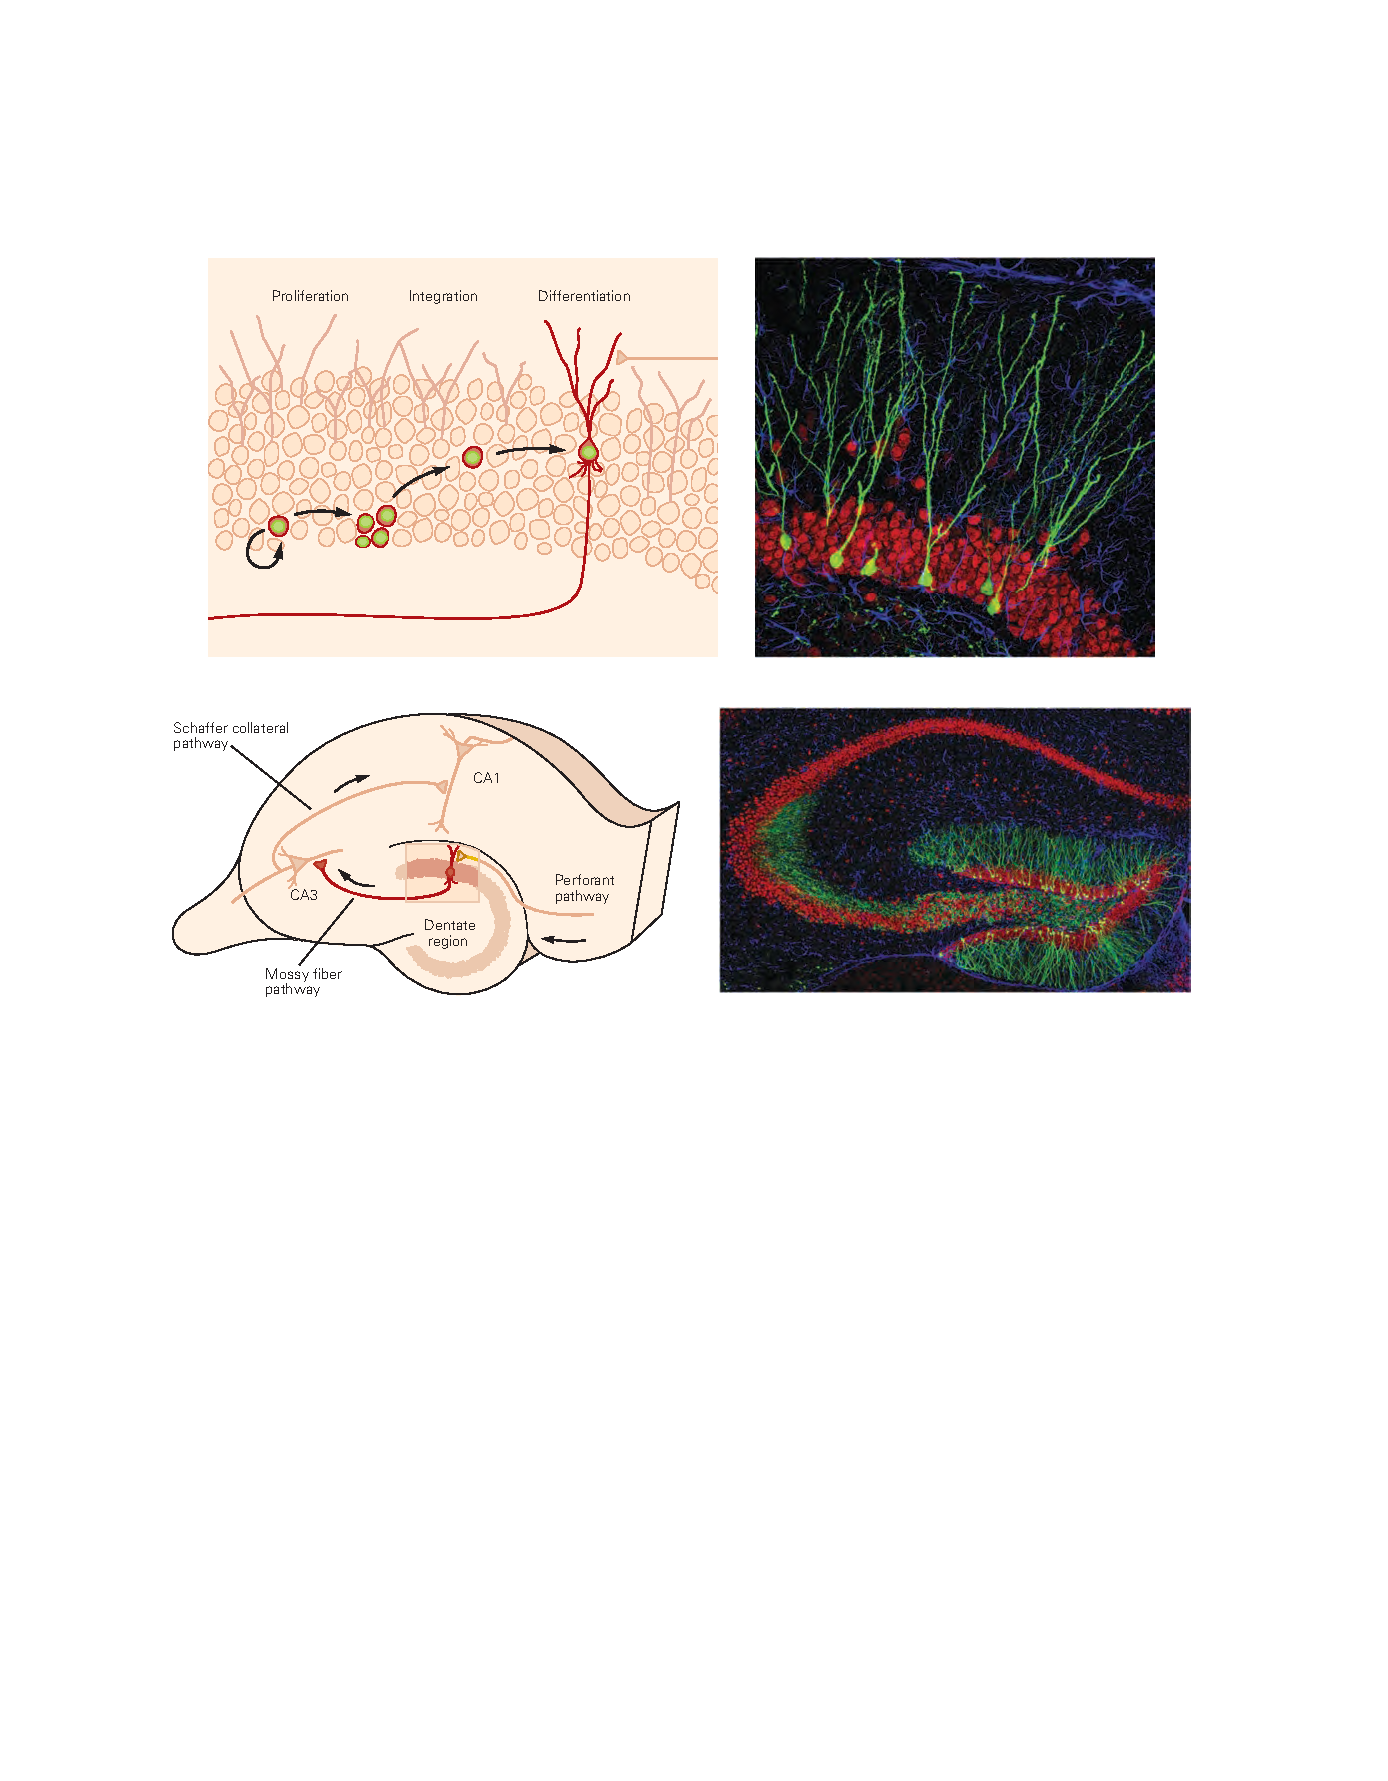
\includegraphics[width=1.0\linewidth]{chap50/fig_50_12}
	\caption{出生于成年啮齿动物齿状回生发区的神经元被整合到海马回路中。
		左图显示了神经元分化和整合到齿状回回路中的途径。
		右边的图像显示了新生成的神经元和它们的树突状乔木,它们用表达绿色荧光蛋白的病毒标记。}
	\label{fig:50_12}
\end{figure}


\begin{figure}[htbp]
	\centering
	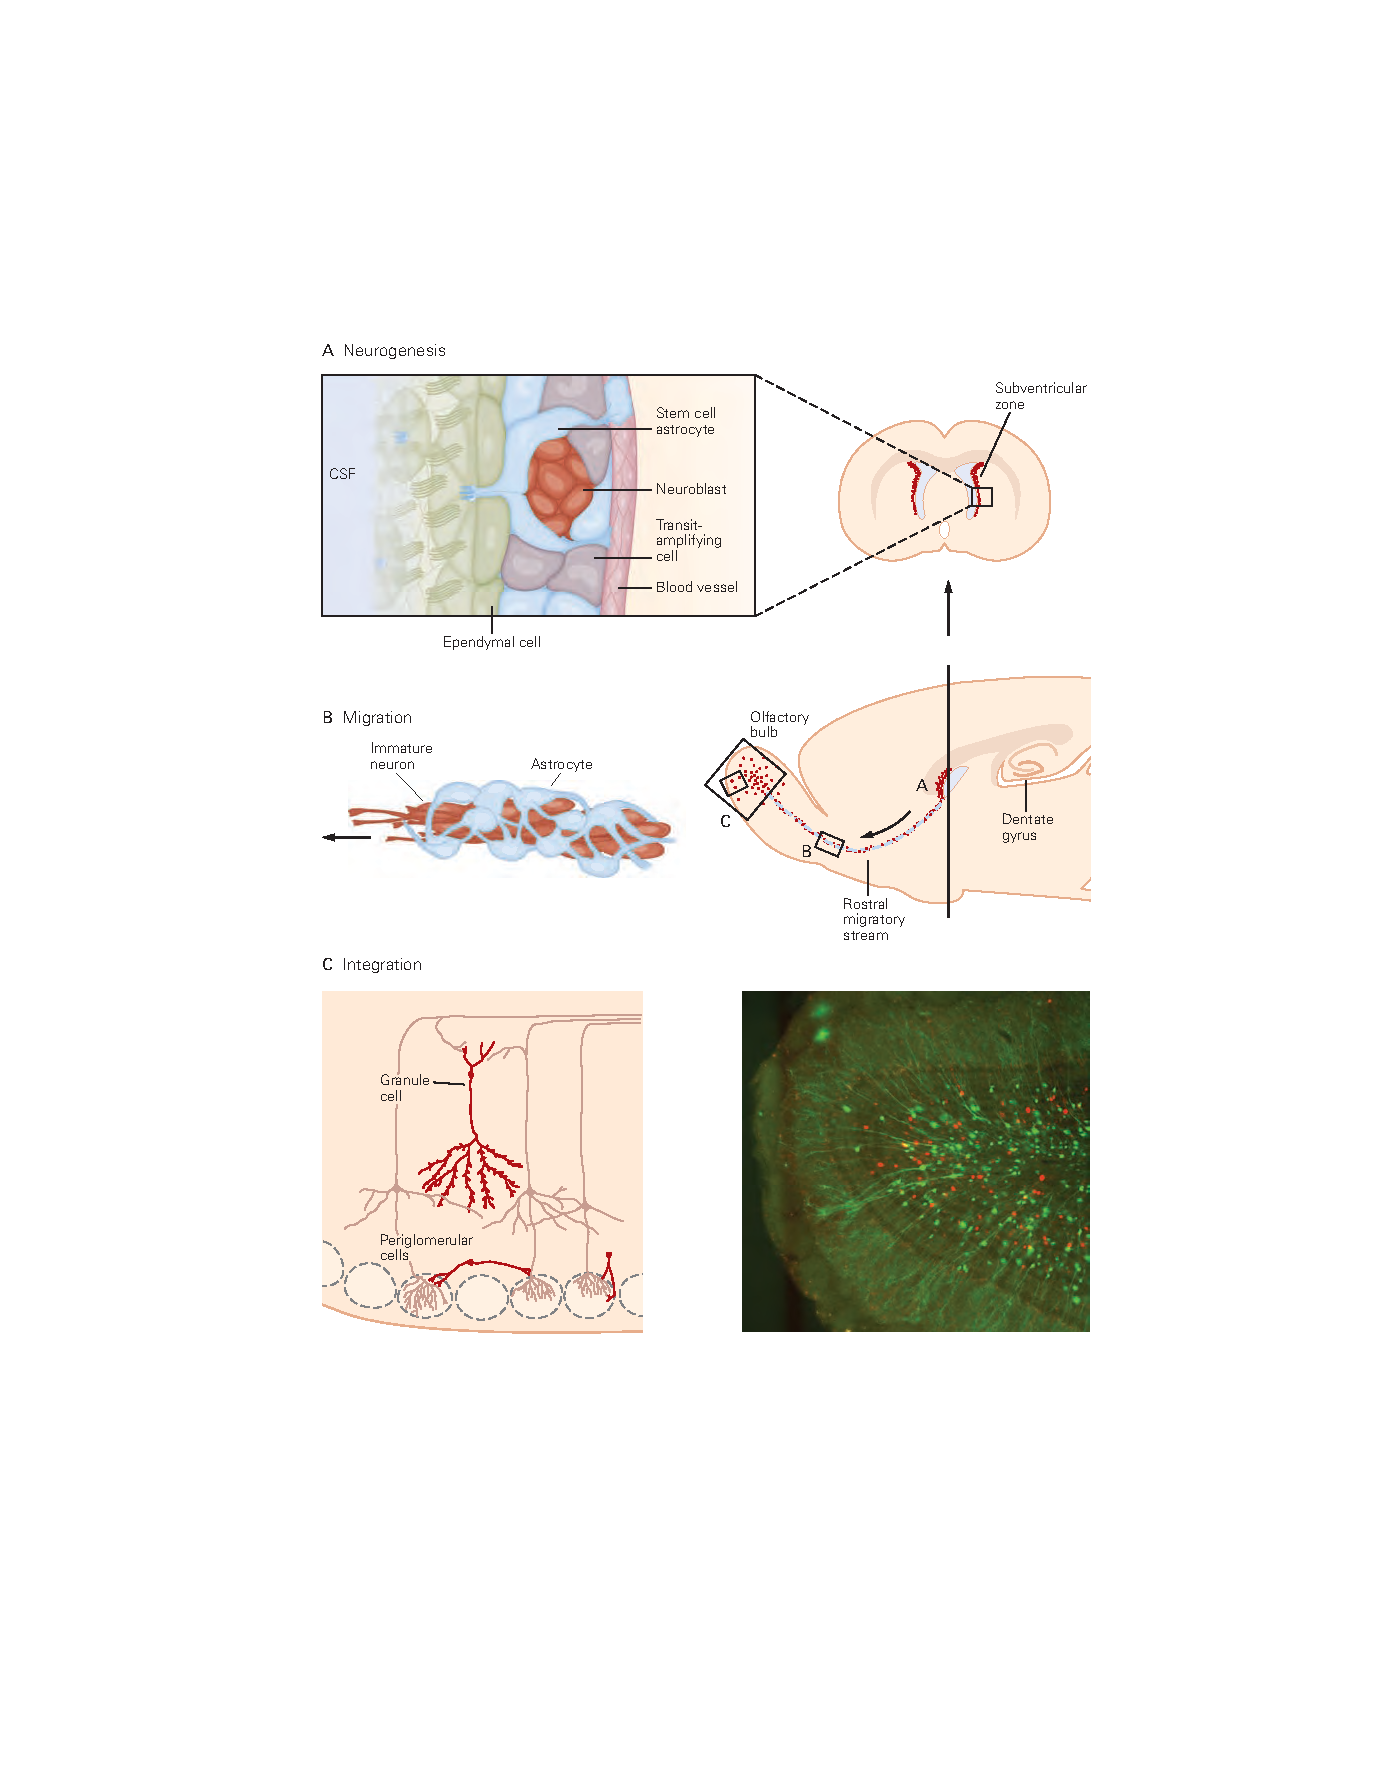
\includegraphics[width=0.87\linewidth]{chap50/fig_50_13}
	\caption{成人脑室区神经元的起源和命运\cite{tavazoie2008specialized}。
		\textbf{A.} 成神经细胞从星形胶质细胞干细胞通过脑室下区靠近血管的局部生态位内的细胞群有序发展。
		\textbf{B.} 成神经细胞分化成未成熟的神经元,这些神经元使用星形胶质细胞作为向导迁移到嗅球。
		它们在称为链迁移的过程中相互爬行。
		\textbf{C.} 到达嗅球后,未成熟的神经元分化为颗粒细胞和球周细胞,两类嗅球中间神经元。}
	\label{fig:50_13}
\end{figure}


成熟动物中出生的神经元的特性尚不完全清楚,但它们似乎能够概括胚胎中出现的神经元的许多特性。
当成人体内新神经元的产生受到阻止时,由嗅球和海马体介导的某些行为就会退化。
相反,一些行为改变伴随着成人神经发生速度的改变。
在抑郁症和慢性压力的动物模型中,成年神经发生可能会减少,而动物栖息地的丰富或久坐不动的啮齿动物的身体活动的增加可以增加新神经元的产生。


哪些细胞会产生成年神经元?
胚胎神经元和神经胶质细胞来自多能祖细胞的原理也适用于成人出生的神经元。
干细胞是成人和胚胎神经元的来源。
它们可能源自放射状神经胶质细胞,放射状神经胶质细胞在胚胎发育过程中也是神经元的来源(第~\ref{chap:chap46}~章)。
这些细胞的一个子集在妊娠期间退出细胞周期,变得静止,并在心室表面附近居住。
在成年期,它们被激活,重新进入细胞周期,并产生神经元。


虽然到目前为止,成人神经发生与受损组织的修复没有直接联系,但它的发现在两个重要方面影响了损伤恢复的研究。
首先,内源性产生的神经元可以通过成年神经细胞的丛林区分和扩展过程,并可以整合到功能回路中,这一发现促使研究人员测试了移植的神经元或前体也是如此的想法。
其次,由于可以诱导神经前体分裂和分化,因此现在正在考虑旨在增强这种先天能力的策略,其目标是产生足够数量的神经元以替代因受伤或神经退行性疾病而丢失的神经元。
正如我们在下面描述的,这些想法在过去几十年里已经从科幻小说发展到非常接近临床试验的成果。



\section{治疗干预可能会保留或替换受伤的中枢神经元}

\subsection{神经元或其祖细胞的移植可以替代丢失的神经元}

多年来,神经学家一直将发育中的神经元移植到实验动物体内,以观察新神经元是否可以逆转损伤或疾病的影响。
这些尝试在一些案例中取得了可喜的成果。


一种是替代在帕金森病中死亡的多巴胺能细胞。
当移植到纹状体中时,这些神经元将多巴胺释放到它们的目标上,而不需要长出长轴突或形成精细的突触(图~\ref{fig:50_14})。
另一种方法是将不成熟的抑制性中间神经元从产生它们的神经节隆起(第~\ref{chap:chap46}~章)移植到皮层,在那里它们成熟并形成突触。
通过增强抑制,这些神经元减弱了抑制驱动力不足发挥作用的疾病的表现,例如癫痫和焦虑症。


\begin{figure}[htbp]
	\centering
	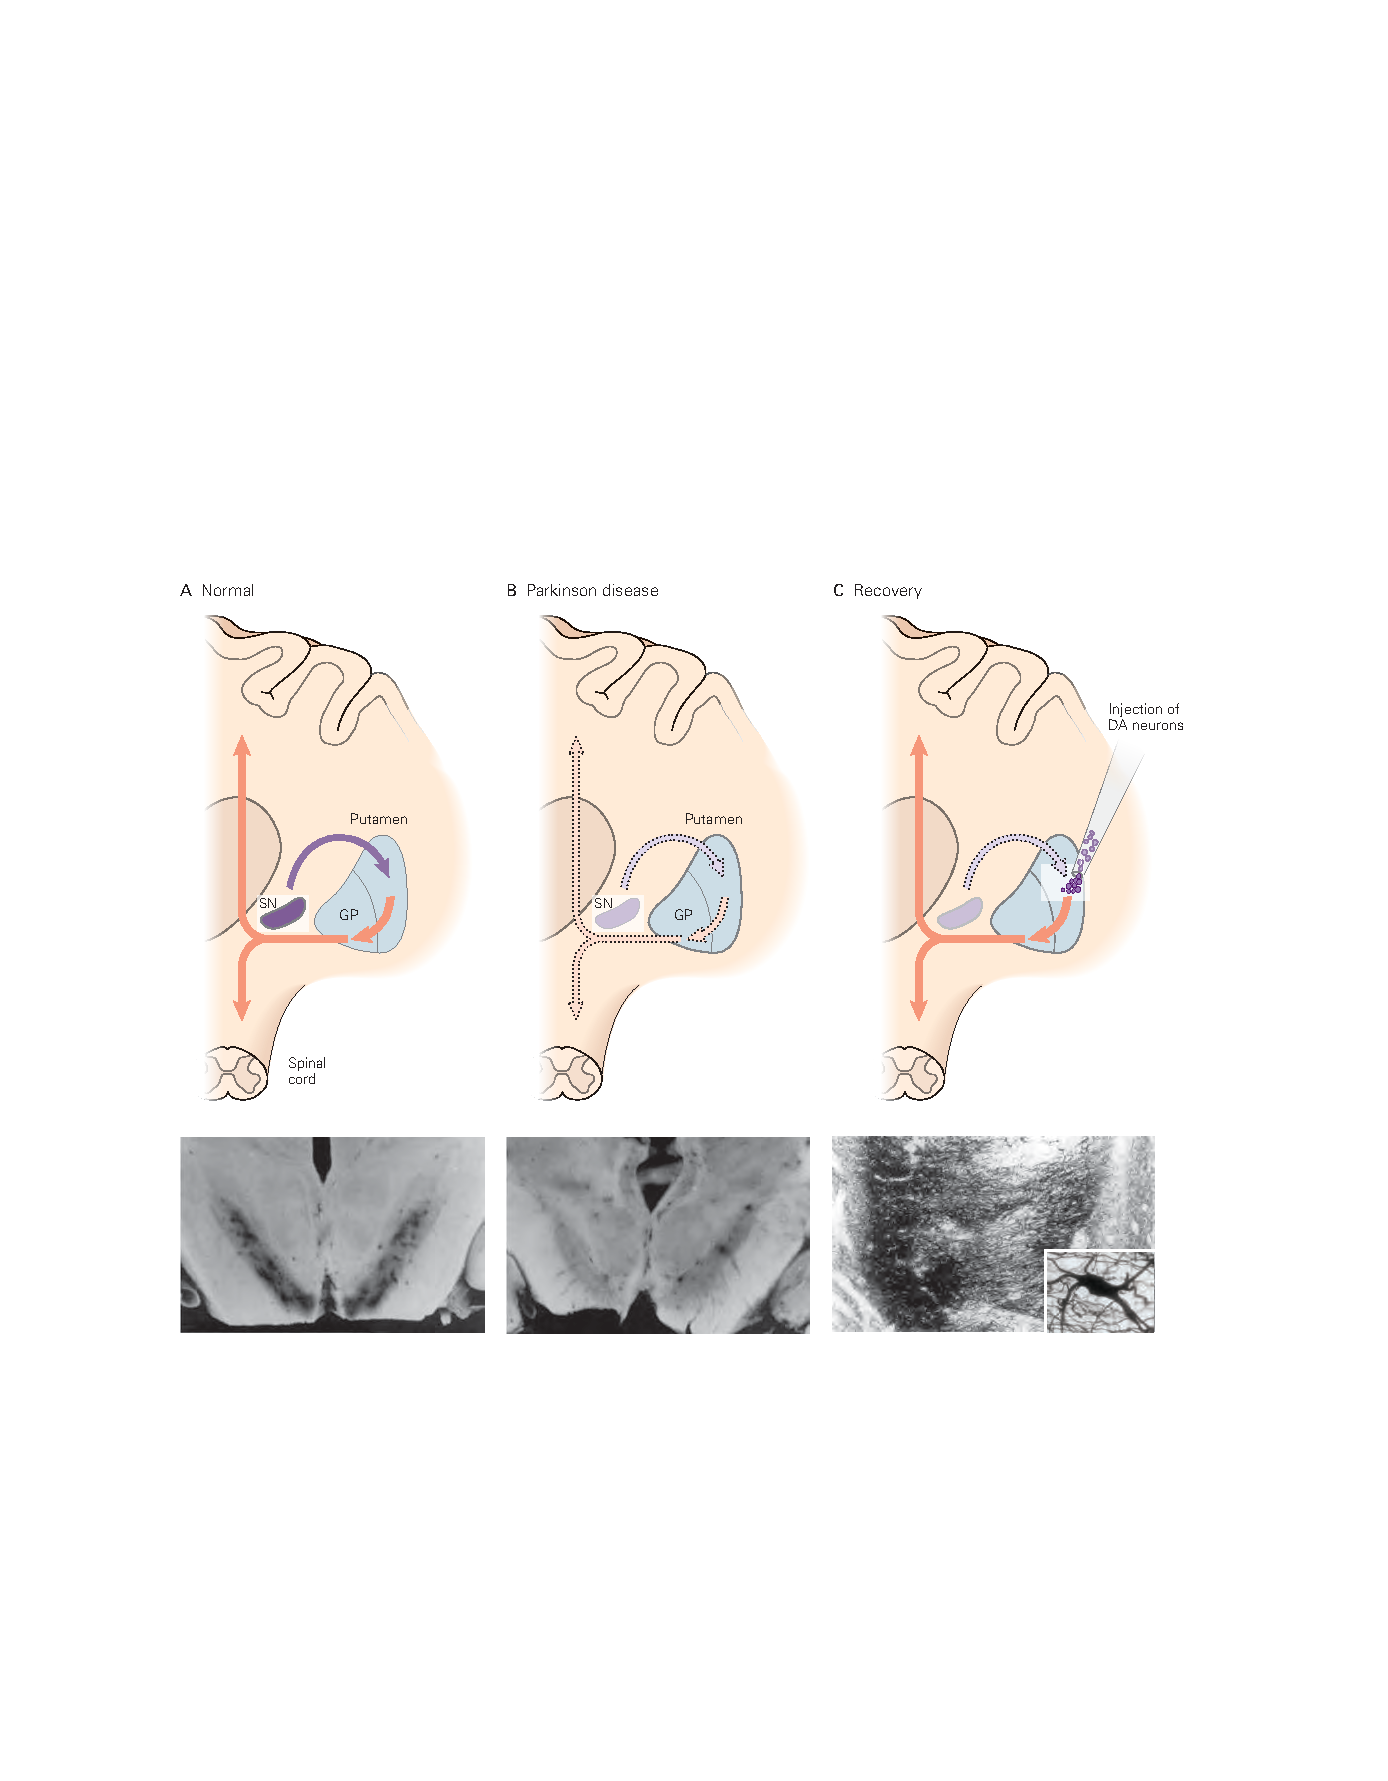
\includegraphics[width=1.0\linewidth]{chap50/fig_50_14}
	\caption{帕金森病中\textit{多巴胺能}神经元的缺失可以通过将胚胎细胞移植到壳核中来治疗。
		\textbf{A.} 在健康的大脑中,来自\textit{黑质}的多巴胺能投射支配壳核,进而激活\textit{苍白球}中的神经元。
		大脑和脊髓的苍白球输出促进运动。
		下图显示了人类黑质中富含黑色素的多巴胺能神经元。
		\textbf{B.} 在帕金森病中,黑质中多巴胺能神经元的丧失剥夺了壳核-苍白球通路的驱动力。
		图表下方的图像显示帕金森病患者的黑质中几乎没有富含黑色素的多巴胺能神经元。
		\textbf{C.} 将胚胎多巴胺能神经元直接注射到壳核中会重新激活苍白球输出通路。
		下图显示了移植到人类患者壳核中的胚胎中脑多巴胺能神经元的细胞体和轴突中的酪氨酸羟化酶表达\cite{kordower2000neuropathology}。}
	\label{fig:50_14}
\end{figure}


不幸的是,将这些方法应用于人类患者一直充满困难。
一个是难以获得足够数量和足够纯度的发育中的神经元。
其次,通过引入新基因来修改神经元以提高它们在新环境中发挥作用的机会一直具有挑战性。
第三,在许多情况下,移植的神经元已经太成熟,无法正确分化或有效整合到功能回路中。


这些障碍可以通过将神经前体移植到成年大脑中来克服,在那里它们可以在适宜的环境中继续分化成神经元。
几类前体细胞已成功移植,包括神经干细胞和定向前体细胞。
\textit{胚胎干细胞}已取得一些初步成功。
这些细胞来源于早期胚泡阶段的胚胎,可以产生身体的所有细胞。
因为它们可以在培养中无限分裂,所以可以产生大量细胞,诱导分化,然后移植。


最近,通过对皮肤成纤维细胞进行分子重编程以创建\textit{诱导的多能性干细胞}(图~\ref{fig:50_15}),该技术得到了增强。

这些细胞与\textit{胚胎干细胞}相比具有明显的优势;
它们的生产不需要胚胎,有效地绕过了阻碍使用人类\textit{胚胎干细胞}进行研究的实际、政治和伦理问题的雷区。
\textit{诱导的多能性干细胞}的另一个优势是它们可以从个体患者自身的皮肤细胞中产生,巧妙地避免了免疫不相容的问题。
还可以通过在移植前修复缺陷基因来对培养的\textit{诱导的多能性干细胞}进行基因修饰。


\begin{figure}[htbp]
	\centering
	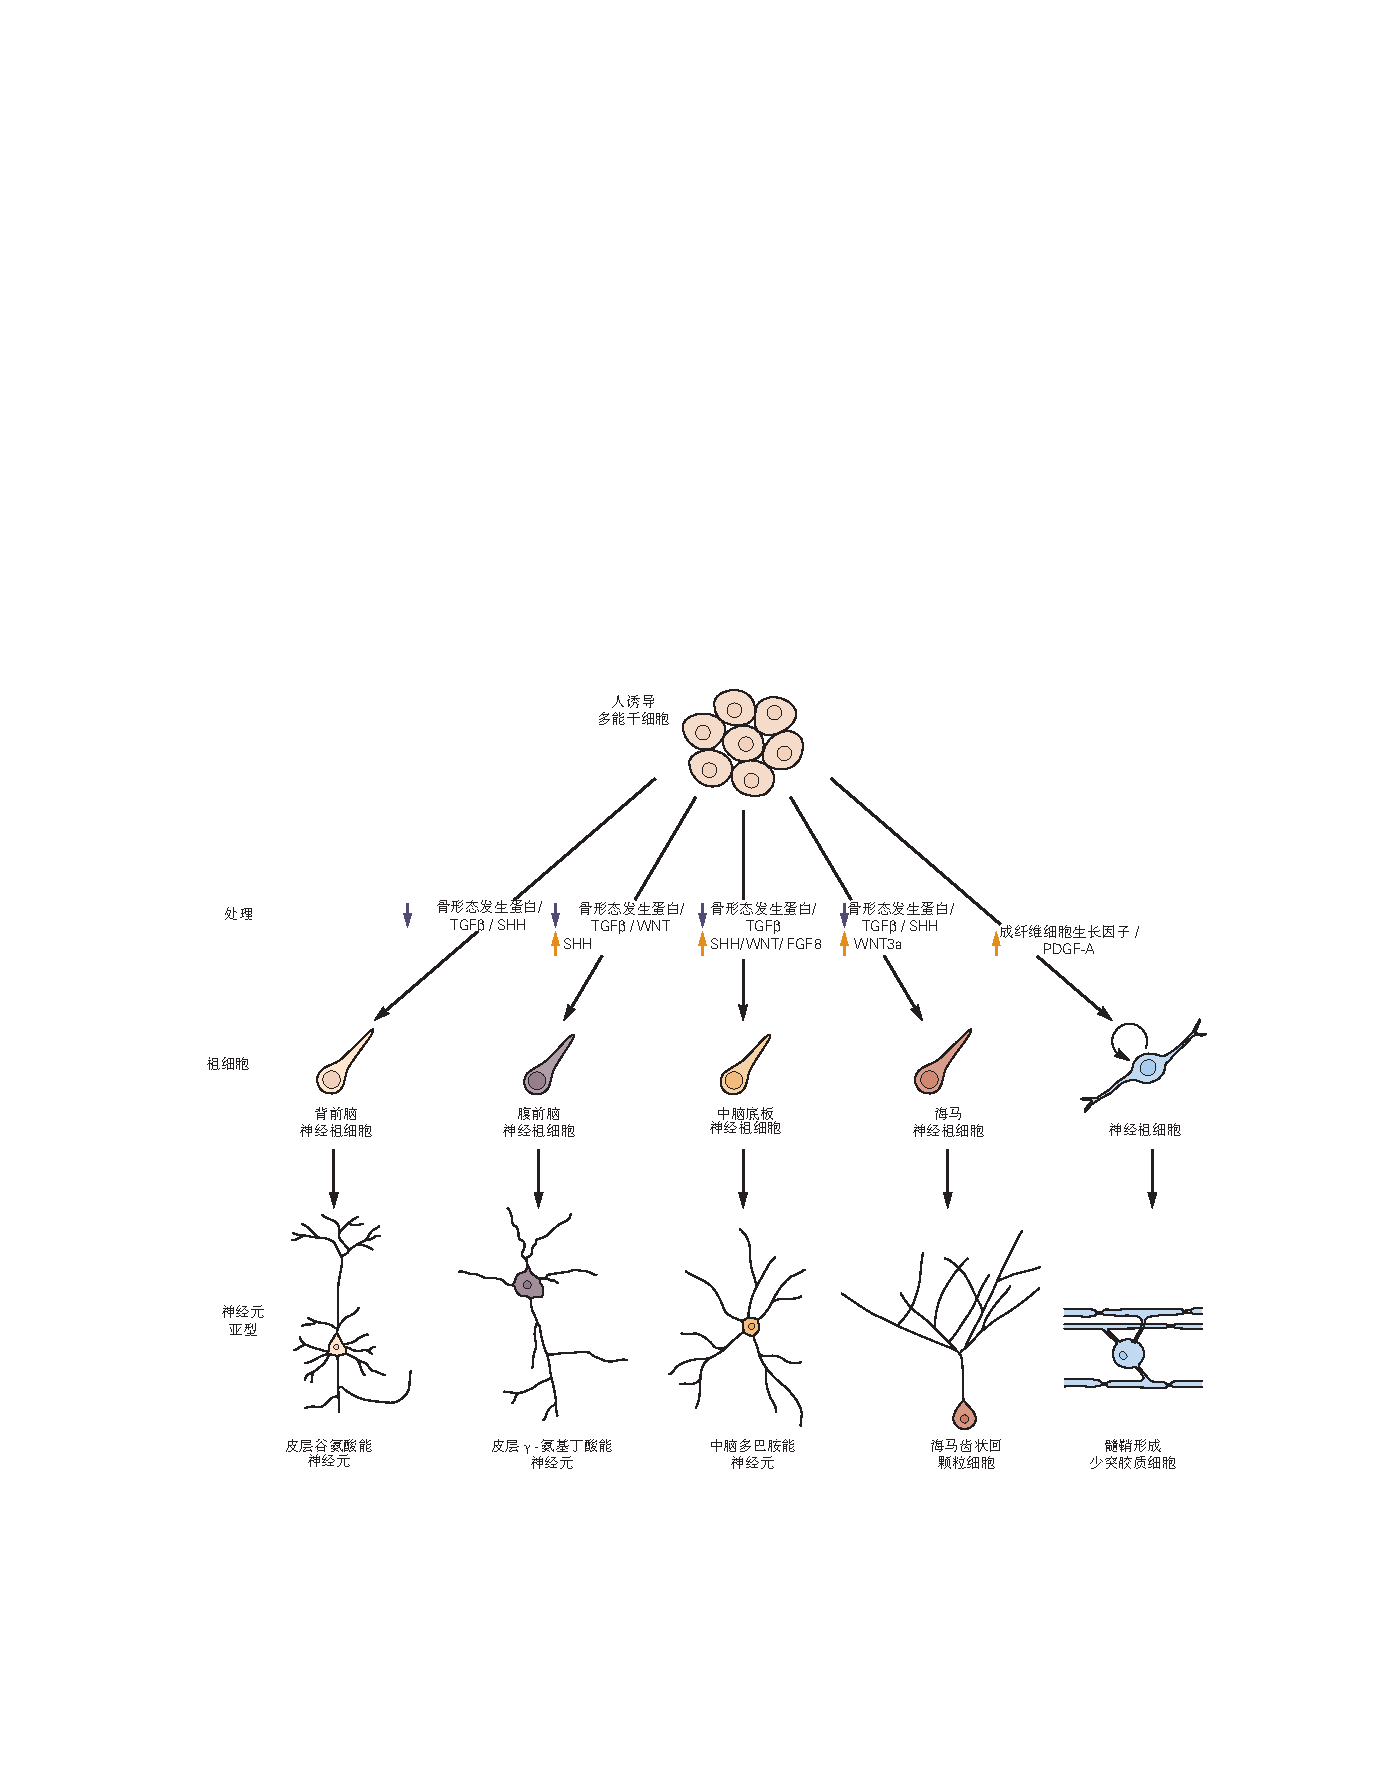
\includegraphics[width=1.0\linewidth]{chap50/fig_50_15}
	\caption{诱导多能干细胞可以重新编程以产生许多神经元和神经胶质类型的前体。
		然后可以将前体移植到大脑或脊髓中,细胞在那里完成分化并整合到功能回路中\cite{wen2016modeling}。}
	\label{fig:50_15}
\end{figure}


由于\textit{胚胎干细胞}和\textit{诱导的多能性干细胞}具有产生任何细胞类型的潜力,因此在移植之前,它们的分化必须沿着特定的培养途径进行引导。
现在已经设计出从\textit{胚胎干细胞}和\textit{诱导的多能性干细胞}生成特定类别的神经前体、神经元和神经胶质细胞的方法(图~\ref{fig:50_15})。
例如,可以生成具有在肌萎缩性侧索硬化症中丧失的脊髓运动神经元的许多或全部特性的神经元(图~\ref{fig:50_16}),或者生成在帕金森病中从纹状体中丧失的多巴胺能神经元,然后 将这些神经元移植到脊髓或大脑中。


\begin{figure}[htbp]
	\centering
	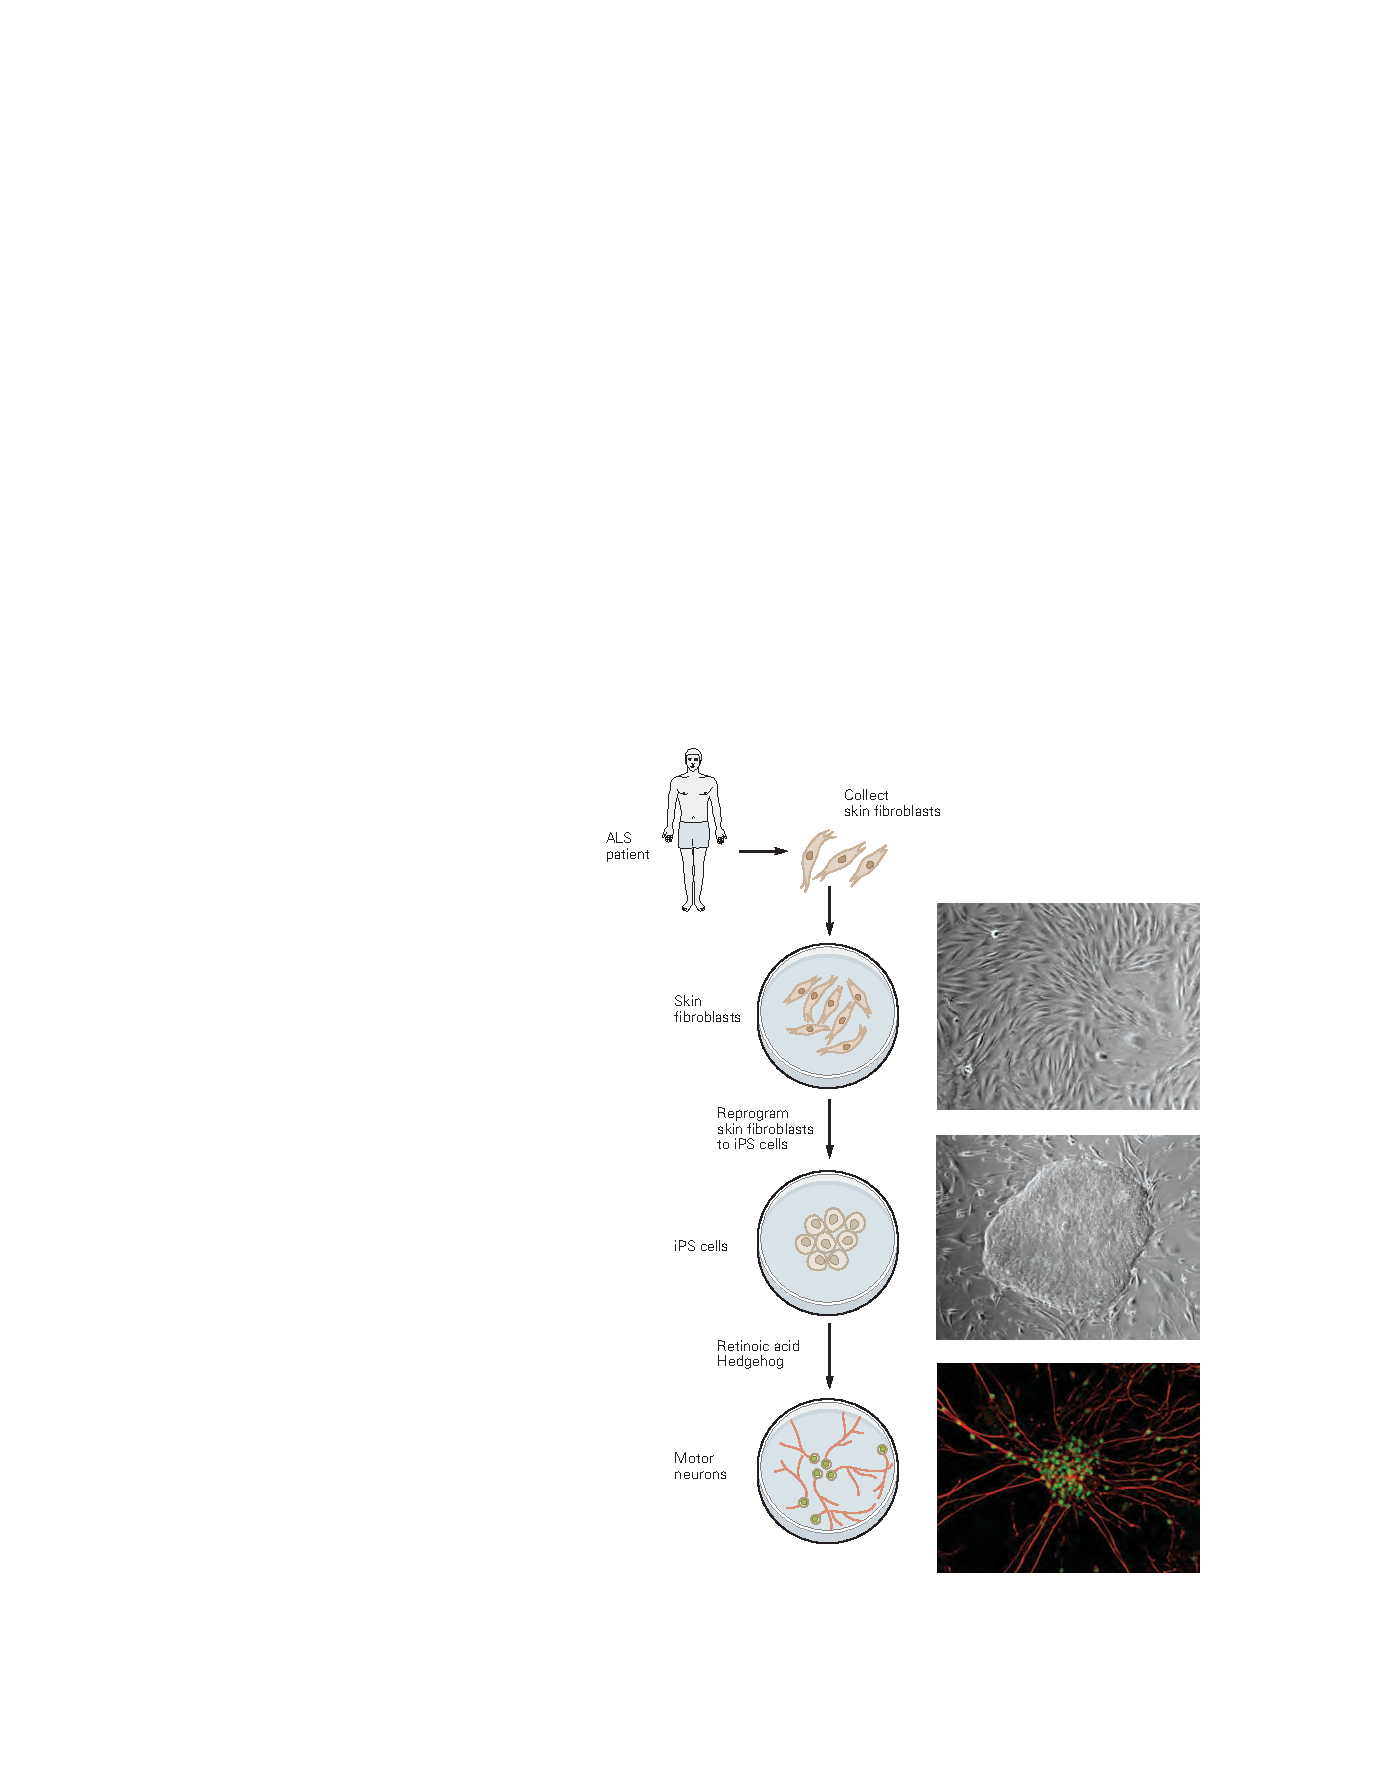
\includegraphics[width=0.77\linewidth]{chap50/fig_50_16}
	\caption{来自患有\textit{肌萎缩侧索硬化}的个体的诱导多能干细胞可以分化为脊髓运动神经元。
		来自\textit{肌萎缩侧索硬化}患者皮肤的成纤维细胞用于生成\textit{诱导的多能性干细胞},然后将其定向至运动神经元命运(见图~\ref{fig:50_15})。
		这些细胞可用于分析\textit{肌萎缩侧索硬化}中运动神经元丢失的机制。
		右图显示(从上到下)培养的成纤维细胞、\textit{诱导的多能性干细胞}细胞团和表达特征性核转录因子(绿色)和轴突蛋白(红色)的分化运动神经元。}
	\label{fig:50_16}
\end{figure}


尽管需要克服许多障碍,但使用\textit{胚胎干细胞}和\textit{诱导的多能性干细胞}细胞衍生神经元的临床试验正在进行中。
此外,这些细胞还被用于化学筛选,以鉴定能够抵消人类神经退行性疾病背后的细胞缺陷的化合物。



\subsection{刺激损伤区域的神经发生可能有助于恢复功能}

如果在成人受伤后,可以刺激内源性神经元前体产生能够替代那些已经丢失的神经元的神经元呢?
最近的两组研究结果表明,这个想法并非遥不可及。


首先,能够在培养物中形成神经元的前体已从成人神经系统的许多部分分离出来,包括大脑皮层和脊髓,尽管成人的神经发生通常局限于嗅球和海马体。
这种细胞命运的转变导致了这样的想法,即成人的神经发生只发生在少数几个部位,因为只有它们包含适当的允许或刺激因素。
这一假设激发了对此类因素的研究,希望它们可以用于呈现更大范围的能够支持神经发生的位点。


其次,在少数情况下,即使在大脑皮层或脊髓等神经发生通常不会发生的区域,外伤或缺血性损伤(类似于中风)也会刺激新神经元的产生。
中风和受伤后恢复较差的事实表明,自发代偿性神经发生(如果发生在人类身上)不足以进行组织修复。
然而,损伤诱导的神经发生在实验动物中以多种方式得到增强。
其中之一,生长因子的施用促进了在培养物中生长的祖细胞的神经元产生。
另一方面,保留分裂能力的胶质细胞,例如视网膜中的 Müller 胶质细胞或皮层中的星形胶质细胞,被重新编程以分化为神经元。
如果此类干预措施适用于人类,则需要更换的神经元范围将大大增加。



\subsection{非神经元细胞或其祖细胞的移植可以改善神经元功能}

脑损伤后神经元以外的细胞会丢失。
损失最严重的是少突胶质细胞,即围绕中央轴突形成髓鞘的细胞。
髓鞘的剥离在外伤后很长时间内仍在继续,并导致可能未直接受伤的轴突功能逐渐丧失。


尽管成人大脑和脊髓能够产生新的少突胶质细胞并替换丢失的髓鞘,但在许多情况下,这种产生不足以恢复功能。
由于几种常见的神经系统疾病,尤其是多发性硬化症,都伴随着严重的脱髓鞘状态,因此人们对为神经系统提供额外的少突胶质细胞前体以增加髓鞘再生产生了浓厚的兴趣。


神经干细胞、多能祖细胞、\textit{胚胎干细胞}和\textit{诱导的多能性干细胞}细胞不仅可以产生神经元,还可以产生非神经细胞,包括少突胶质细胞及其直接前体细胞。
事实上,目前,人类\textit{胚胎干细胞}正被导入少突胶质细胞祖细胞,并植入实验动物受伤的脊髓中。
分化为少突胶质细胞的移植细胞可增强髓鞘再生并显著提高实验动物的运动能力(图~\ref{fig:50_17})。


\begin{figure}[htbp]
	\centering
	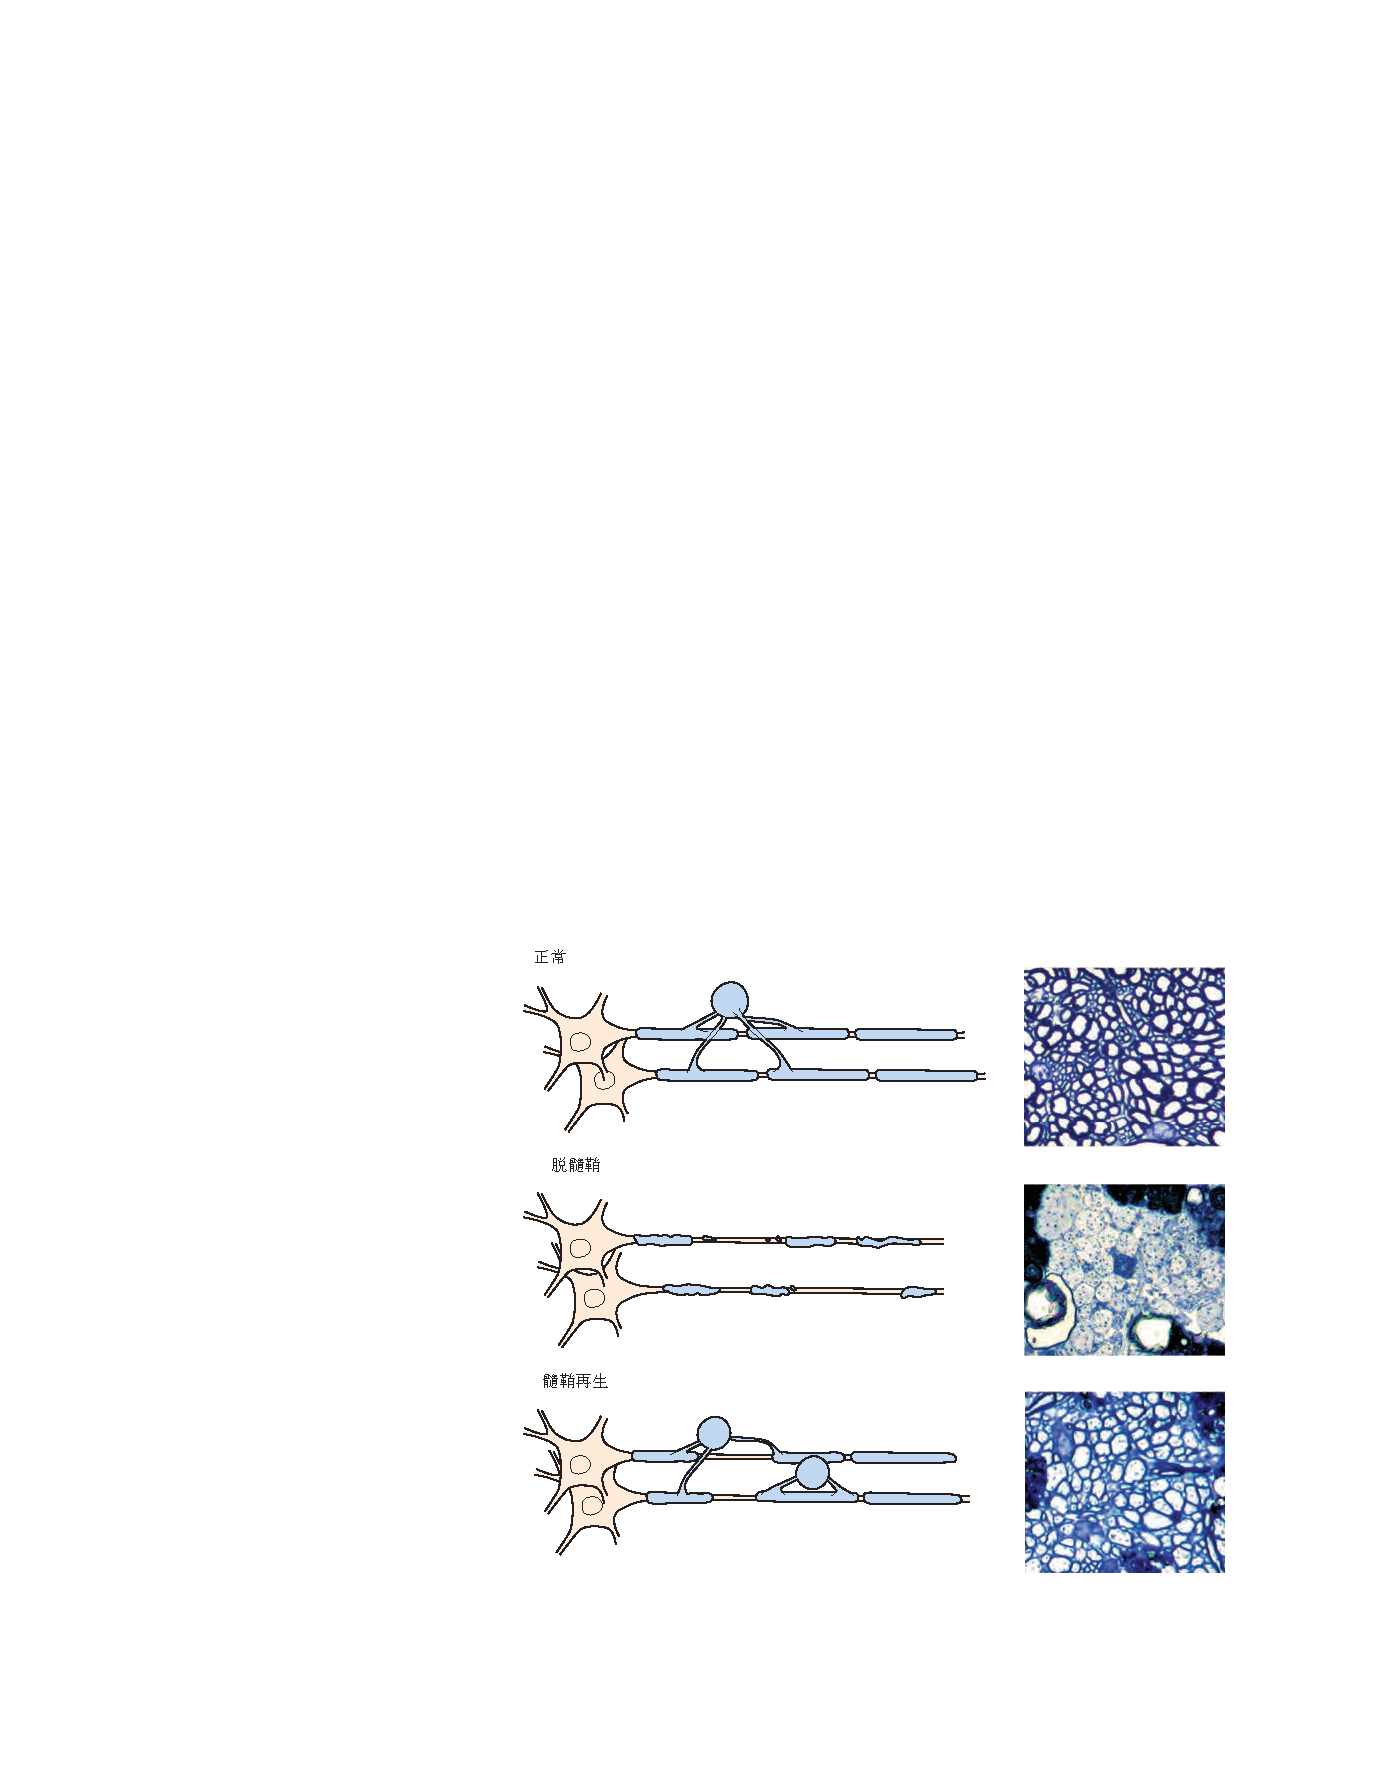
\includegraphics[width=0.8\linewidth]{chap50/fig_50_17}
	\caption{通过移植的少突胶质细胞干细胞恢复中枢神经系统的髓鞘形成。
		在轴突脱髓鞘的啮齿动物中,少突胶质前体细胞的移植物可以使髓鞘形成恢复到接近正常水平。
		右图显示了通过中枢神经束的切片\cite{franklin2008remyelination}。}
	\label{fig:50_17}
\end{figure}


\subsection{功能恢复是再生疗法的目标}

我们需要记住,如果这些轴突不能与它们的靶细胞形成功能性突触,那么更换中枢神经元或增强轴突再生的努力将毫无用处。
因此,关于成人轴突再生的相同基本问题也适用于突触发生:它会发生吗?
如果不会,为什么不呢?


解决这些问题一直很困难,因为实验性损伤后的轴突再生通常很差,以至于轴突永远无法到达适当的目标区域。
然而,本章前面讨论的几项研究提供了希望,即在致密的成人神经细胞内可能形成突触。
事实上,受伤后再生的轴突分支可以在附近的目标上形成突触。
例如,\textit{阿瓜约}和他的同事发现,当视网膜轴突通过已移植到视神经的周围神经时,它们能够重新长成上丘(图~\ref{fig:50_18}A)。
值得注意的是,当眼睛被照亮时,一些丘神经元会发射动作电位,表明功能性突触连接已经重新建立(图~\ref{fig:50_18}B)。
如上所述,最近的研究通过增强其内在生长程序促进了切断的轴突的再生,并观察到一些功能恢复。


\begin{figure}[htbp]
	\centering
	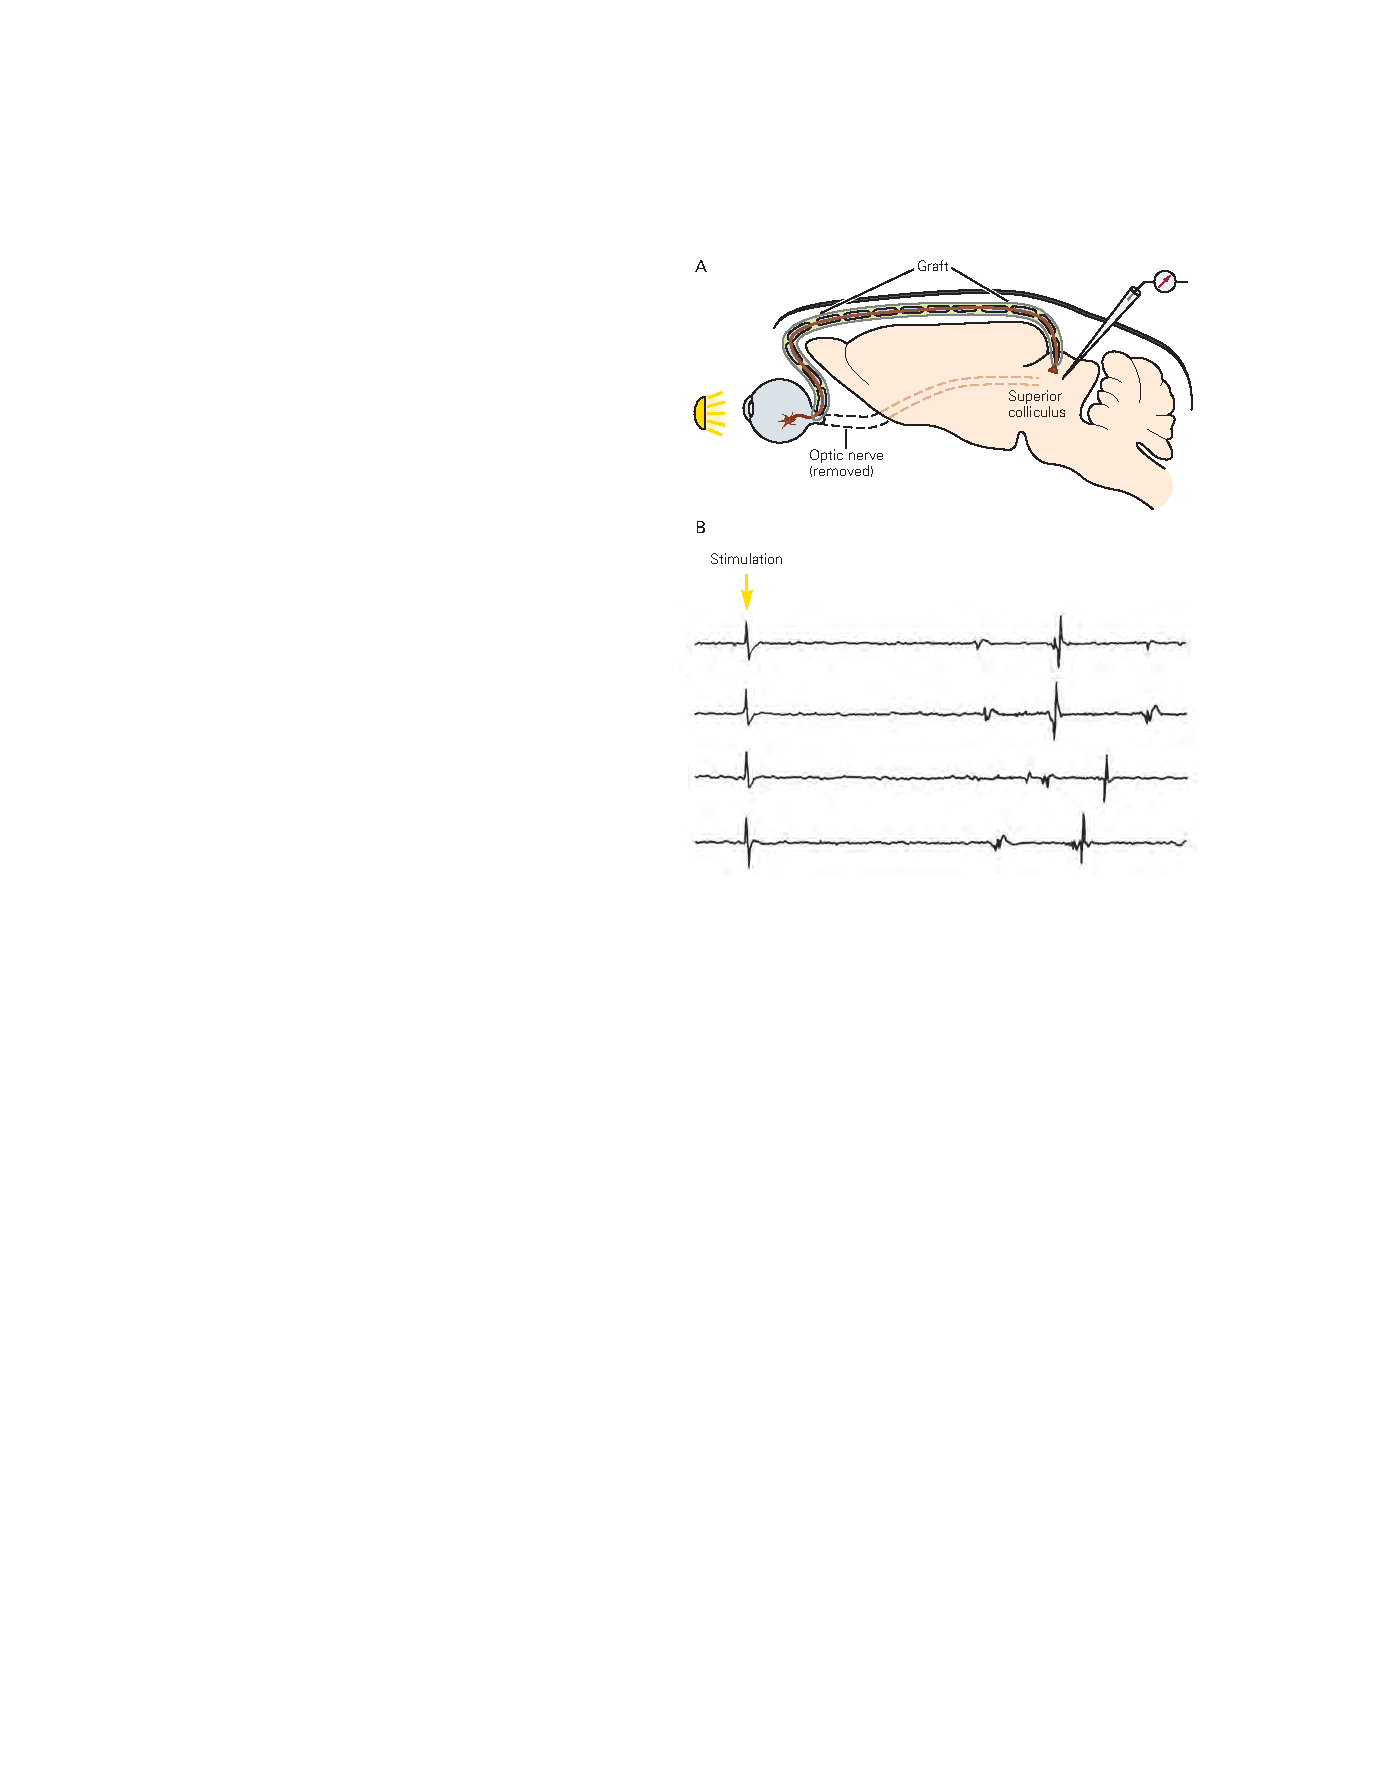
\includegraphics[width=0.7\linewidth]{chap50/fig_50_18}
	\caption{视神经中再生的视网膜神经节轴突可以形成功能性突触\cite{keirstead1989electrophysiologic}。
		\textbf{A.} 移除成年大鼠的一段视神经,并在其位置移植一段坐骨神经。
		坐骨神经的另一端与上丘相连。
		一些视网膜神经节细胞轴突通过坐骨神经再生并进入上丘。
		\textbf{B.} 一旦视网膜神经节神经元的轴突再生,就从上丘进行记录。
		传送到眼睛的闪光在丘脑神经元中引起动作电位,表明至少一些再生的轴突已经形成了功能性突触。}
	\label{fig:50_18}
\end{figure}


同样,内源性产生或由研究人员植入的神经元可以形成和接收突触。
因此,有理由相信,如果可以诱导受伤的轴突再生,或者提供新的神经元来替换丢失的轴突,它们将以有助于恢复丢失的功能和行为的方式连接起来。



\section{要点}

1. 当轴突被横切时,远端节段发生退化,这一过程称为沃勒变性。
近端节段和细胞体也会发生变化,受损神经元的突触输入和目标也会发生变化。


2. 长期以来,人们一直认为沃勒变性是远端节段被剥夺细胞体营养的被动和不可避免的结果,但它是一个主动的、受调节的过程并不为人所知。
称为\textit{烟酰胺单核苷酸腺嘌呤转移酶1}和 SARM1 的基因是控制该过程的核心信号通路的关键组成部分。
对该通路的干预可以减缓甚至停止退化。 


3. 轴突在受伤后可以再生并形成新的突触,但在哺乳动物中,外周轴突的再生比中央轴突的再生更为广泛和有效。


4. 外周轴突和中央轴突反应不同的一个关键因素是,受伤的中央轴突所处的环境不利于生长。
它既缺乏周围神经通路中存在的营养因子,又含有周围神经中不存在的生长抑制因子。


5. 抑制再生的结构包括在华勒变性后持续存在的髓鞘碎片和在损伤部位形成神经胶质疤痕的星形胶质细胞。
髓鞘中的抑制因子包括 Nogo 和髓鞘相关糖蛋白。
星形胶质细胞分泌的抑制因子包括硫酸软骨素蛋白聚糖。
 

6. 由于在发育过程中活跃的生长程序下调,成人中枢神经元生长的内在能力下降也阻碍了中枢再生。
恢复或解除抑制生长途径的干预措施,例如\textit{两面神激酶-信号转导和转录激活因子}和\textit{哺乳动物雷帕霉素靶蛋白}信号,可以促进再生。


7. 然而,重要的是要注意,受伤后再生失败可能与关键时期结束时发生的连接稳定有关。
例如,主要发生在关键期末期的髓鞘形成可能具有防止突触连接进一步大规模重排的次要作用。
因此,需要谨慎确保旨在促进损伤后恢复的治疗不会最终促进适应不良回路的形成。 


8. 损伤后恢复功能的另一种方法是利用完整轴突形成新连接的能力,产生适应性回路,在一定程度上补偿因损伤而丧失的轴突。 


9. 所有神经发生都发生在妊娠期间或妊娠后不久的传统观点现在已经被新神经元在整个生命过程中的几个大脑区域中诞生的发现所修正。
这些神经元来自常驻干细胞,可以整合到功能回路中。


10. 能够形成新神经元的细胞也存在于大脑和脊髓的许多其他区域,但仍处于静止状态。
尝试通过提供生长因子或引入促生长基因(转录重编程)来激活它们,可以利用它们在受伤后或神经退行性疾病中的潜力。


11. 另一种神经元替代方法是植入发育中的神经元。
尽管有时在实验动物中将胎儿神经元用于此目的,但更有用的来源可能是源自\textit{胚胎干细胞}或\textit{诱导的多能性干细胞}的神经元。
它们可以大量生长,必要时进行基因改造,并进行处理以分化成特定的神经元类型。
使用这种方法的临床研究现已开始。



